\documentclass{mathnotes}
\usepackage{mathnotes}

% % Necessary commands.
\newcommand{\thetitlename}{Ecuaciones en Derivadas Parciales}
\newcommand{\thetitle}{\HRule \thetitlename\\\HRule Notas no revisadas\footnote{Se agradecen sugerencias, correcciones, etc. Seguramente haya más cosas mal que páginas.}}
\newcommand{\theauthor}{Guillermo Ruiz Álvarez}
\newcommand{\thedate}{2015}

\begin{document}
\maketitle
\newpage
\tableofcontents
\newpage

\section{El principio del máximo}
\subsection{El principio del máximo unidimensional}

Esta sección comienza con el estudio del principio del máximo unidimensional en ecuaciones diferenciales.
\begin{mathresult}{Principio del máximo unidimensional}
Dada la inecuación 
\begin{equation}
\label{eq:principio-del-maximo}
-u''+g(x)u'+h(x)u(x) < 0 \ \ \forall x \in (0,1) 
\end{equation}
Si $h(x) \ge 0$ en el intervalo $(0,1)$, la solución de \eqref{eq:principio-del-maximo} no puede tener un máximo (local o global) no negativo en dicho intervalo.
\end{mathresult}
\begin{proof}
Sea $u$ la solución de \eqref{eq:principio-del-maximo}. Supongamos que $u$ tiene un máximo no negativo, es decir, $\exists c\in (0,1)$ que satisface $u(c) \ge u(x) \ \forall x \in (0,1)$ con $u(c)\ge 0$.
Si esto es así, la solución de la inecuación cumple $u'(c)=0$ y $u''(c) \le 0$. De aquí se obtiene:
$$\underbrace{-u''(c)}_{\ge 0}+\underbrace{g(c)u'(c)}_{=0}+\underbrace{h(c)u(c)}_{\ge 0} \ge 0$$
El tercer término es no negativo dado que, por hipótesis, $h(x) \ge 0$ en todo el intervalo y $u(c)$ es no negativo.
Esto nos lleva a una contradiccion con \eqref{eq:principio-del-maximo}, por tanto, $\nexists c \in (0,1)$ que satisfaga $u(c) \ge u(x) \ \forall x \in (0,1)$ con $u(c)\ge 0$.
\end{proof}
\see El resultado es cierto para cualquier intervalo abierto acotado, no sólo para $(0,1)$.

A partir del resultado anterior, se va a dar la prueba del siguiente teorema:

\begin{theorem}\label{theorem1}
Sea $u\in C^2(0,1)$ que satisface
\begin{equation}\label{eq:principio-del-maximo2}
-u''(x)+g(x)u'(x)+h(x)u(x) \le 0
\end{equation}
con $g, h$ acotadas y $h(x) \ge 0$ en cualquier subintervalo de $(0,1)$.

Entonces, si $\exists a\in (0,1)$ tal que $u(a) \ge u(x) \ \forall x\in(0,1)$ y $u(a) \ge 0$ (i.e. u alcanza un máximo no negativo en $a$), se tiene que $u = cte$ en $(0,1)$.
\end{theorem}
\begin{proof}
Sea $u$ la solución de \eqref{eq:principio-del-maximo2}. Supongamos que $u$ es una función no constante. Sabemos que $\exists b \in (0,1)$ tal que $u(b) < u(a)$ dado que $a$ es un máximo (local o global) de $u$ y $u$ es no constante. Supongamos $0< a < b < 1$.\footnote{Para el caso contrario la demostración es similar.}

Construimos la función
$$\varphi(x) = e^{\alpha(x-a)}-1$$

\begin{figure}[h]
\centering

\begin{tikzpicture}
	\draw[->] (-3,0) -- (3,0) node[right] {$x$};
	\draw[->] (0,-1) -- (0,3) node[above] {$y$};
	\draw[-]  (1, 0.1) -- (1, -0.1) node[below] {$a$};
	\draw[-]  (0.5, 0.1) -- (0.5, -0.1) node[below] {$\frac{a}{2}$};
	\draw[] (-0.2,0) node[below] {$0$};
	\draw[-]  (2, 0.1) -- (2, -0.1) node[below] {$1$};
	\draw[scale=1,domain=-1:2.3,smooth,variable=\x,blue] 
		plot ({\x},{exp(\x-1)-1})
		node[right] {$\varphi(x)$};
\end{tikzpicture}

\label{fig:phi-x}
\caption{Función $\varphi$}
\end{figure}

Si aplicamos \eqref{eq:principio-del-maximo2} a $\varphi$ obtenemos 

\begin{align*}
-\varphi''(x)+g(x)\varphi'(x)+h(x)\varphi(x) & \le 0 \numberthis \label{eq:phi-estricta}\\
e^{\alpha(x-a)}\left(-\alpha^2+\alpha g(x)\right) + h(x)\underbrace{(e^\alpha(x-a)-1)}_{\varphi} & \le 0\\
e^{\alpha(x-a)}\left(-\alpha^2+\alpha g(x)+\underbrace{h(x)}_{\ge 0}\underbrace{(1-e^{-\alpha(x-a)})}_{\le 1}\right) & \le 0\\
e^{\alpha(x-a)}\left(-\alpha^2 + \alpha g(x) + h(x)\right) & \le 0
\end{align*}

Dado que $g,h$ son acotadas, se puede tomar un valor de $\alpha$ suficientemente grande de forma que $-\alpha^2 + \alpha g(x) + h(x)  < 0$. Es decir, que $\varphi$ cumpla \eqref{eq:phi-estricta} para la desigualdad estricta. Tomamos $\alpha$ tal que la desigualdad estricta para $\varphi$ se cumpla $\forall x \in [\frac{a}{2}, b] \subset (0,1)$

Definimos ahora $$w(x) = u(x) + \varepsilon \varphi(x)$$
con $\varepsilon > 0$

Aplicando \eqref{eq:principio-del-maximo2} a $w$ obtenemos
\begin{align*}
-w'' + g(x)w'+h(x)w = & -u''+g(x)u'+h(x)u\\
& + \varepsilon\left(-\varphi''+g(x)\varphi'+h(x)\varphi\right)\\
\le &\ 0 + \varepsilon\left(-\varphi''+g(x)\varphi'+h(x)\varphi\right)\\
< &\ 0	\numberthis \label{eq:desigualdad-w}
\end{align*}
que se cumple $\forall x \in [\frac{a}{2}, b]$ si tomamos un valor de $\alpha$ adecuado. 
Dado que
\begin{equation*}
\left\{
\begin{array}{l}
w(b) = u(b) + \varepsilon\varphi(b)\\
w(a) = u(a)
\end{array}
\right.
\end{equation*}
 si tomamos $\varepsilon < \frac{u(a)-u(b)}{\varphi(b)}$ tenemos que 
 \begin{equation}\label{eq:wb-menor-wa}
 w(b) < w(a)
 \end{equation}
Además, como 
\begin{equation*}
\left\{
\begin{array}{l l}
w(a) = u(a) & \\
\varphi(x) < 0 & \forall x < a \\
\end{array}
\right.
\end{equation*}
tenemos que $w(x) = u(x) + \varepsilon\varphi(x) < u(x) < u(a) = w(a)$, 
es decir, 
\begin{equation}\label{eq:wx-menor-wa}
w(x) < w(a)
\end{equation}
en todo el intervalo $[\frac{a}{2}, a)$.

\noindent\textbf{Conclusión:}
\begin{itemize}
\item Utilizando \eqref{eq:desigualdad-w} y las hipótesis del teorema, obtenemos, para $w$, las hipótesis del \textbf{Principio del máximo}.
\item Vemos que $w$ tiene un máximo no negativo en el intervalo $[a, b)$, puesto que
\begin{itemize}
\item a la izquierda de $a$ tenemos \eqref{eq:wx-menor-wa}
\item a la derecha de $a$ tenemos \eqref{eq:wb-menor-wa}
\end{itemize}
Como $u$ es continua, tal y como está definida, $w$ también es continua. Se tiene entonces que $\exists c \in [a, b) \subset (\frac{a}{2}, b)$ tal que $w(c) = max\ w(x)$ en dicho intervalo. Es decir, $w$ alcanza un máximo no negativo, contradiciendo el teorema.
\end{itemize}
\newpage
Tenemos por tanto una contradicción, habiendo partido de las hipótesis del teorema y de la suposición de que $u$ es no constante.
\end{proof}

\corol
Sean $g,h$ acotadas y $u\in C[0,1] \cap C^2(0,1)$ una función no constante que satisface \eqref{eq:principio-del-maximo2}. 

Sea $M = \max_{x \in [0,1]}\ u(x)$. Sea $m = max\{u(0), u(1)\}$. Se tiene que:
\begin{itemize}
\item Si $M \ge 0 \implies u(x) < M\ \forall x\in(0,1)$
\item $u(x) < max\{0,m\}\ \forall x\in(0,1)$.
\end{itemize}

\begin{proof}
Dado que $[0,1]$ es un compacto y $u\in C[0,1]$, se tiene que $u$ alcanza un máximo $M$ en dicho intervalo.

\begin{itemize}
\item Caso $M<0$.

Como $M$ es un máximo de $u$, se cumple que $u(x) \le M < 0\ \forall x\in[0,1]$. Por tanto $u(x) < max\{0, m\}$.

\item Caso $M\ge 0$. 

Como $M$ es un máximo de $u$, se tiene que $m \le M$.

En las hipótesis del corolario tenemos que $u$ es no constante. Dado que $M$ es un máximo no negativo, no puede alcanzarse en el interior de $[0,1]$, porque si fuese así, por el teorema, $u$ sería constante. Así, el máximo se alcanza en $[0,1]\setminus(0,1)$ por lo que $m = M$.

Es decir, $u(x) < M = m = max\{0, m\}\ \forall x\in (0,1)$.
\end{itemize}
\end{proof}

Si suponemos, por ejemplo, que el máximo se alcanza en $x=0$. La solución de la ecuación, en un entorno de $0$, podría ser como se muestra en la figura \ref{fig:sol-entorno-cero}. Vamos a ver que condiciones son necesarias para que el caso de la figura \ref{fig:sol-entorno-cero-a}, en el que la tangente a la función es horizontal en el $0$, sea imposible.

\begin{figure}[ht]
\centering
\begin{subfigure}{.5\textwidth}
	\centering
  	\begin{tikzpicture}
		\draw[->] (-1,0) -- (3,0) node[right] {$x$};
		\draw[->] (0,-1) -- (0,3) node[above] {$y$};
		\draw[] (-0.2,0) node[below] {$0$};
		\draw[-, blue, dashed, scale=2] (0,1) -- (0.7,1);
		\draw[scale=2,domain=0:0.7,smooth,variable=\x,blue] 
			plot ({\x},{-(\x*\x)+1})
			node[right] {$u(x)$};
	\end{tikzpicture}
	\caption{}
	\label{fig:sol-entorno-cero-a}
\end{subfigure}%
\begin{subfigure}{.5\textwidth}
	\centering
  	\begin{tikzpicture}
		\draw[->] (-1,0) -- (3,0) node[right] {$x$};
		\draw[->] (0,-1) -- (0,3) node[above] {$y$};
		\draw[] (-0.2,0) node[below] {$0$};
		\draw[scale=2,domain=0:0.7,dashed,variable=\x,blue] 
			plot ({\x},{-0.4*\x+1});
		\draw[scale=2,domain=0:0.6,smooth,variable=\x,blue] 
			plot ({\x},{-(\x*\x)-0.4*\x+1})
			node[right] {$u(x)$};
	\end{tikzpicture}
	\caption{}
	\label{fig:sol-entorno-cero-b}
\end{subfigure}%

\caption{Función $u$ en un entorno de $0$}
\label{fig:sol-entorno-cero}
\end{figure}

\newpage
\begin{theorem}\label{theorem2}
Sea $u\in C^2(0,1)$ no constante que satisface \eqref{eq:principio-del-maximo2} y 
\begin{equation*}
\left\{
\begin{array}{l l}
u(0) \ge u(x) & \forall x \in (0,1)\\
u(0) \ge 0
\end{array}
\right.
\end{equation*}
es decir, $u$ alcanza un máximo no negativo en $0$.
Sea $h(x) \ge 0$.

Si $g(x) + xh(x)$ está acotada superiormente en un entorno de $0$, entonces
$$\lim_{x\to0^+}u'(x) < 0$$
\end{theorem}

\begin{proof}
Dado que $u$ es no constante $\exists a\in (0,1)$ tal que $u(a) < u(0)$.
Consideremos $\varphi(x) = e^{\alpha x}-1$. 

\begin{figure}[h]
\centering

\begin{tikzpicture}
	\draw[->] (-3,0) -- (3,0) node[right] {$x$};
	\draw[->] (0,-1) -- (0,3) node[above] {$y$};
	\draw[-]  (1, 0.1) -- (1, -0.1) node[below] {$a$};
	\draw[] (-0.2,0) node[below] {$0$};
	\draw[-]  (2, 0.1) -- (2, -0.1) node[below] {$1$};
	\draw[scale=1,domain=-1:1.3,smooth,variable=\x,blue] 
		plot ({\x},{exp(\x)-1})
		node[right] {$\varphi(x)$};
\end{tikzpicture}

\label{fig:phi2-x}
\caption{Función $\varphi$}
\end{figure}

Tenemos que
\begin{align*}
-\varphi''(x)+g(x)\varphi'(x)+h\varphi & = \\
e^{\alpha x}\left\{-\alpha^2 +\alpha g(x)+\underbrace{h(x)}_{\ge 0}\left(\underbrace{1-e^{-\alpha x}}_{\text{concava }(\le ax)}\right)\right\} & \le\\
e^{\alpha x}\left\{-\alpha^2+\alpha g(x) + \alpha xh(x)\right\} & = \\
\alpha e^{\alpha x}\{-\alpha + \left(\underbrace{g(x) +xh(x)}_{\text{acotado superiormente}}\right)\} & < 0
\end{align*}
es decir
$$-\varphi''(x)+g(x)\varphi(x)+h\varphi < 0$$
para un valor de $\alpha$ adecuado. Definimos ahora
$$w(x) = u(x) +\varepsilon \varphi(x)$$
Tenemos que
\begin{align*}
-w'' + g(x)w'+h(x)w = & -u''+g(x)u'+h(x)u\\
& + \varepsilon\left(-\varphi''+g(x)\varphi'+h(x)\varphi\right)\\
\le &\ 0 + \varepsilon\left(-\varphi''+g(x)\varphi'+h(x)\varphi\right)\\
< &\ 0
\end{align*}
Dado que $w(a) = u(a) + \varepsilon\varphi(a)$, si tomamos $\varepsilon < \frac{u(0)-u(a)}{\varphi(a)}$, se cumple que $w(a) < u(0) = w(0)$.
Tenemos por tanto que $w(a) \le w(x)\ \forall x \in [0, a]$. Obtenemos, $$\lim_{x\to0^+}w'(x) \le 0$$
Para ver la desigualdad estricta, basta con derivar $w$:
$$w'(x) = u'(x) +\varepsilon\varphi'(x)$$
Sabemos que $\varphi'(x) = \alpha e^{\alpha x}$, por tanto $\varphi'(0) = \alpha$.
Con esta información, tenemos
$$\lim_{x\to0^+} w(x) = \lim_{x\to0^+} u(x) +\varepsilon \alpha \le 0$$
Es decir, $$\lim_{x\to0^+} u(x) \le -\varepsilon \alpha < 0$$
\end{proof}

Vamos a ver la necesidad de que $g(x)$ y $g(x) + xh(x)$ sean acotadas para el teorema \ref{theorem1} y \ref{theorem2}, respectivamente. Veámoslo con un contraejemplo. Supongamos que
\begin{equation*}
g(x) = 
\left\{
\begin{array}{l l}
3/x & x\neq 0\\
0 & x = 0
\end{array}
\right.
\end{equation*}


\begin{figure}[ht]
\centering
\label{fig:g-de-x}
\begin{tikzpicture}
	\draw[->] (-3,0) -- (3,0) node[right] {$x$};
	\draw[->] (0,-3) -- (0,3) node[above] {$y$};
	\draw [fill, blue] (0,0) circle [radius=.05];
	\draw[scale=1,domain=-3:-1,smooth,variable=\x,blue] 
		plot ({\x},{3/(\x)});
	\draw[scale=1,domain=1:3,smooth,variable=\x,blue] 
		plot ({\x},{3/(\x)})
		node[right] {$g(x)$};
\end{tikzpicture}
\caption{Función $g$}
\end{figure}

Sea $u(x) = 1-x^4$ y $h(x) = 0$. Vemos que $u$ cumple
\begin{equation*}
\left\{
\begin{array}{l l}
-u''(x) + g(x)u'(x) = 0 & \forall x\in(-1,1)\\
u(0)=1 > u(x) & \forall x\in(-1,1)\\
\end{array}
\right.
\end{equation*}

Sin embargo, si observamos la figura \ref{fig:sol-contraejemplo-pm} vemos que no se cumplen ninguno de los dos teoremas anteriores.
\begin{itemize}
\item En el caso en el que consideremos la función en el intervalo $(-1,1)$, vemos que $u$ presenta un máximo no negativo en $(0,1)$. (Ver figura \ref{fig:sol-contraejemplo-pm1}). No se cumple el teorema \ref{theorem1} por no estar $g(x)$ acotada.
\item En el caso en el que consideremos la función en el intervalo $(0,1)$, vemos que $\lim_{x\to0^+}u(x) = 0$ (Ver figura \ref{fig:sol-contraejemplo-pm2}). No se cumple el teorema \ref{theorem2} por no estar $g(x)+xh(x)$ acotada.
\end{itemize}

\begin{figure}[ht]
\centering
\begin{subfigure}{.5\textwidth}
	\centering
  	\begin{tikzpicture}
		\draw[->] (-2,0) -- (2,0) node[right] {$x$};
		\draw[->] (0,-1) -- (0,1.5) node[above] {$y$};
		\draw[-] (-1,0.1) -- (-1,-0.1) node[below] {$-1$};
		\draw[-] (1,0.1) -- (1,-0.1) node[below] {$1$};
		\draw[scale=1,domain=-1:1,smooth,variable=\x,blue] 
			plot ({\x},{sqrt(1-\x*\x)})
			node[above right] {$u(x)$};
	\end{tikzpicture}
	\caption{}
	\label{fig:sol-contraejemplo-pm1}
\end{subfigure}%
\begin{subfigure}{.5\textwidth}
	\centering
  	\begin{tikzpicture}
		\draw[->] (-1,0) -- (2,0) node[right] {$x$};
		\draw[->] (0,-1) -- (0,1.5) node[above] {$y$};
		\draw[-, dashed, blue] (0,1) -- (1.5,1);
		\draw[] (-0.2,0) node[below] {$0$};
		\draw[-] (1,0.1) -- (1,-0.1) node[below] {$1$};
		\draw[scale=1,domain=0:1,smooth,variable=\x,blue] 
			plot ({\x},{sqrt(1-\x*\x)})
			node[above right] {$u(x)$};
	\end{tikzpicture}
	\caption{}
	\label{fig:sol-contraejemplo-pm2}
\end{subfigure}%

\caption{Función $u$}
\label{fig:sol-contraejemplo-pm}
\end{figure}

\newpage
\subsection{El principio del máximo n-dimensional}
\begin{mathresult}{Principio del máximo n-dimensional}
Dada la inecuación
\begin{equation}\label{eq:principio-del-maximo-Ndim}
-\Delta u(x) + \sum_{i=1}^n g_i(x)\frac{du(x)}{dx_i}+h(x)u(x) < 0 \ \ \forall x\in\Omega
\end{equation}

Sea $u\in C^2(\Omega)$ la solución de \eqref{eq:principio-del-maximo-Ndim}.
Si $h(x) \ge 0$, $u$ no puede alcanzar un máximo no negativo en $\Omega$.
\end{mathresult}
\see $\Delta u(x)$ es el laplaciano de $u(x)$ y se define como sigue:
$$\Delta u(x) = \sum_{i=1}^n\frac{d^2u(x)}{d^2x_i}$$

$\nabla u(x)$ es el gradiente de $u(x)$ y se define como sigue:
$$\nabla u(x) = \left(\frac{du(x)}{dx_1}, \hdots, \frac{du(x)}{dx_n}\right)^T$$
\begin{proof}
Sea $x_0\in \Omega$ y $u$ la solución de \eqref{eq:principio-del-maximo-Ndim}. Supongamos que $u$ alzanca un máximo no negativo en $x_0$, es decir, $u(x_0) \ge 0$ y $u(x_0) > u(x)\ \forall x \in \Omega$.

Definimos 
\begin{equation*}
\begin{array}{l r l l}
f: & (-\varepsilon, \varepsilon) \subset\mathbb{R} & \longrightarrow  & \mathbb{R}\\
& t & \longrightarrow & f(t) = u(x_0+t\xi)\\
\end{array}
\end{equation*}
con $\xi\in\mathbb{R}^n$.
Se puede observar que $f(0)$ es un máximo para $f$, por tanto
\begin{equation}
\left\{
\begin{array}{l}
f'(0) = 0\\
f''(0) \le 0\\
\end{array}
\right.
\end{equation}

Vamos a analizarlo por partes:
\begin{itemize}
\item $f'(0) = \nabla u(x_0)\xi$. Tenemos entonces que $\nabla u(x_0) = \vec{0}$
\item $f''(0) = \sum_{i,j=1}^n \xi_i\xi_j\frac{d^2u(x_0)}{dx_idx_j} = \xi^T\nabla^2u(x_0)\xi$. De donde se obtiene que $\nabla^2u(x_0) \le 0$. Es decir, $\nabla^2u(x_0)$ es semidefinida negativa.
\end{itemize}

Si tomamos $\xi_i = (0,\hdots, \underbrace{1}_{\text{posición i}}, \hdots, 0)^T$, obtenemos
$$\xi_i^T\nabla^2u(x_0)\xi_j = \Delta u(x_0)$$
Se tiene entonces que $\Delta u(x_0) \leq 0$.
Vamos a analizar ahora la inecuación en $x_0$:
\begin{equation}\label{eq:ineq-Ndimensional}
\underbrace{-\Delta u(x_0)}_{\ge 0} + \sum_{i=1}^n g_i(x_0)\underbrace{\frac{du(x_0)}{dx_i}}_{=0}+\underbrace{h(x_0)}_{\ge 0}u(x_0) \ge 0
\end{equation}

\noindent\textbf{Conclusión:}
Partiendo de las hipótesis del teorema, y suponiendo que $u(x_0)$ es un máximo no negativo, llegamos a \eqref{eq:ineq-Ndimensional}, que supone una contradicción con \eqref{eq:principio-del-maximo-Ndim}.
\end{proof}

\subsection{Principio débil del máximo}
\begin{mathresult}{Principio débil del máximo}
Dada la inecuación
\begin{equation}\label{eq:theorem3}
-\Delta u(x) + \sum_{i=1}^n g_i(x)\frac{du(x)}{dx_i}+h(x)u(x) \le 0 \ \ \forall x\in\Omega
\end{equation}
Sea $\Omega$ un \textbf{dominio} en $\mathbb{R}^n$.
Sea $u\in C(\overline{\Omega})\cap C^2(\Omega)$ la solución de \eqref{eq:theorem3}.
Sean $g_1,\hdots, g_n,h$ funciones acotadas.
Entonces:
\begin{itemize}
\item Si $h=0$ en $\Omega \implies \max_{\overline{\Omega}} u(x)$ se alcanza en $\delta\Omega$. 
\item Si $h>0$ en $\Omega \implies sup_{\Omega} u(x) \le max\left\{0, \max_{\delta\Omega} u(x)\right\}$. Es decir, $u$ no puede tener un máximo no negativo en $\Omega$.
\end{itemize}
\end{mathresult}
\newpage
\see
\begin{itemize}
\item Un \textbf{dominio} es un abierto conexo.
\item $\delta\Omega$ se refiere a la frontera de $\Omega$ 
\item $\overline{\Omega}$ al cierre (o adherencia) de $\Omega$.
\end{itemize}
\begin{proof}
\textbf{Caso $h = 0$}

Como $\Omega$ es un dominio, es acotado, (ver figura \ref{fig:omega}). Por tanto podemos suponer que está en una franja (una variable, por ejemplo $x_1$, se restringe). $\Omega \subset \{x\in \mathbb{R}^n: 0 < x_1 < d\}$.

\begin{figure}[ht]
\centering
\begin{tikzpicture}[scale=2]
\path [pattern=north west lines, pattern color=yellow] (0, -1.2) -- (0, 1.7) -- (2.5, 1.7) -- (2.5, -1.2);
\draw[->] (-1,0) -- (3,0) node[right] {$x_1$};
\draw[] (0,0) node[below left] {$0$};
\draw[] (2.5,0) node[below right] {$d$};
\draw [thick, fill=lemonchiffon] 
	(0.4,0) to [out=87,in=160] 
	(1.4,1) to [out=340,in=30]
	(2.25,.15) to [out=220,in=70]
	(1.4,0) to [out=273, in=273]
	(0.4,0);
\draw [->, dashed] (0, -1.2) -- (0, 1.7);
\draw [->, dashed] (2.5, -1.2) -- (2.5, 1.7);
\draw [] (1.3,1) node[below=3mm] {$\Omega$};

\end{tikzpicture}
\caption{Dominio $\Omega$}
\label{fig:omega}
\end{figure}
Consideramos la función $\varphi(x) = e^{\alpha x_1}$.
Si tomamos un valor de $\alpha$ suficientemente grande, tenemos:
\begin{equation}\label{eq:prueba1-ndim}
-\Delta\varphi + \sum_{i=1}^ng_i(x)\frac{d\varphi}{dx_i} = \alpha e^{\alpha x_1}\left(-\alpha + \underbrace{g_1(x)}_{\text{acotada}}\right) < 0
\end{equation}
Definimos ahora $w(x) = u(x) + \varepsilon\varphi(x)$, que cumple
\begin{align*}
-\Delta w + \sum_{i=1}^{n}g_i(x)\frac{dw}{dx_i} & \le\\
0 + \varepsilon\left(-\Delta\varphi + \sum_{i=1}^{n}g_i(x)\frac{d\varphi}{dx_i}\right) & \underbrace{<}_{\text{\eqref{eq:prueba1-ndim}}} 0
\end{align*}
A partir de la definición de $w$, dado que $\varepsilon, \varphi > 0$, se tiene que:

\begin{equation*}
\begin{array}{l l l l}
u(x) & < & u(x) + \varepsilon\varphi(x) & \\
u(x) & < & w(x) & \forall x \in \Omega\\
\end{array}
\end{equation*}
Como $w$ cumple las hipótesis del \textbf{Principio del máximo n-dimensional}

\begin{equation*}
\begin{array}{l l l}
w(x)_\Omega & < & \max_{\delta\Omega} w(x) \\
w(x)_\Omega & < &  w(c) = u(c) + \epsilon\varphi(c)
\end{array}
\end{equation*}
para algún $c\in\delta\Omega$. Más precisamente

\begin{equation*}
\begin{array}{l l l}
w(x)_\Omega & < & \max_{\delta\Omega}u(x) + \varepsilon e^{\alpha d}
\end{array}
\end{equation*}
Si $\varepsilon\to0$
$$u(x)_\Omega < \max_{\delta\Omega}u(x)$$
es decir, el máximo de la función se alcanza en la frontera de $\Omega$.

\noindent\textbf{Caso $h \ge 0$}

Sea $\Omega_+ = \{x\in \Omega: u(x) > 0\} \equiv$ abierto (ver figura \ref{fig:omega-mas}).

\begin{figure}[ht]
\centering
\begin{tikzpicture}[scale=2]
\draw [->, thick] (0.4, 1.1) -- (1.1, 0.5);
\path [fill=lemonchiffon] 
	(1.4,1) to [out=340,in=30]
	(2.25,.15) to [out=220,in=70]
	(1.4,0) to [out=190, in=130]
	(1.4,1);
\draw [thick] 
	(0.4,0) to [out=87,in=160] 
	(1.4,1) to [out=340,in=30]
	(2.25,.15) to [out=220,in=70]
	(1.4,0) to [out=273, in=273]
	(0.4,0);
\draw [dashed, thick]
	(1.4, 0) to [out=190, in=130]
	(1.4, 1) node[above] {$\delta\Omega\cap\Omega = \{x\in R^n: u(x) = 0\}$};
\draw [] (1.6,0.5) node[below] {$\Omega_+$};
\end{tikzpicture}
\caption{Dominio $\Omega$}
\label{fig:omega-mas}
\end{figure}

\noindent Sea $u$ la solución de 
\begin{equation*}
\begin{array}{l l}
-\Delta u + \sum_{i=0}^ng_i(x)\frac{du}{dx_i} + h(x)u(x)\le0 & \text{en } \Omega_+
\end{array}
\end{equation*}
por la definición de $\Omega_+$ y por ser $h(x) \ge 0$, se tiene $h(x)u(x) \ge 0$, por tanto, 

\begin{equation*}
\begin{array}{l l}
-\Delta u + \sum_{i=0}^ng_i(x)\frac{du}{dx_i} \le -h(x)u(x) \le 0 & \text{en } \Omega_+\\
-\Delta u + \sum_{i=0}^ng_i(x)\frac{du}{dx_i} \le 0 & \text{en } \Omega_+\\
\end{array}
\end{equation*}
En $\Omega_+$ se cumplen las hipótesis del primer apartado del teorema ($u$ cumple la inecuación cuando $h=0$), el cual ya se ha probado. Se tiene
$$\max_{\overline{\Omega}_+}u = \max_{\delta\Omega_+}u$$
y a partir de aquí
$$\max_{\delta\Omega_+}u \le \max_{\delta\Omega}u $$
En la parte de la frontera de $\Omega_+$ que está en $\Omega$ (la que aparece con línea discontinua en la figura \ref{fig:omega-mas}), $u$ es nula, resultando

\begin{equation*}
\left.
\begin{array}{l l}
\text{Si } x\in\overline{\Omega}_+ & 0\le u(x)\le \max_{\delta\Omega}\\
\text{Si } x\in\Omega\setminus\overline{\Omega}_+ & u(x) < 0
\end{array}
\right\}
u(x) \le \max\left\{0, \max_{\delta\Omega} u\right\}
\end{equation*}
\end{proof}

\see
A partir de aquí, se denotará
$$\mathcal{L}(u) = -\Delta u(x) + \sum_{i=1}^n g_i(x)\frac{du(x)}{dx_i} + h(x)u(x)$$
que es un funcional lineal:
\begin{itemize}
\item $\mathcal{L}(u+v) = \mathcal{L}(u) + \mathcal{L}(v)$
\item $\mathcal{L}(\lambda u) = \lambda\mathcal{L}(u)$
\end{itemize}

\newpage
\begin{mathresult}{Lema de Hopf}
Sea $\Omega$ un abierto de $R^n$ y $u\in C^2$ que satisface
\begin{equation*}
-\Delta u(x) + \sum_{i=1}^n g_i(x)\frac{du(x)}{dx_i} + h(x)u(x) \le 0 \ \text{en } \Omega
\end{equation*}
donde $g_1,\hdots,g_n,h$ son acotadas.
Sea $x_0$ un punto de la frontera de $\Omega$ que cumple:
\begin{itemize}
\item $u$ es continua en $x_0$.
\item $u(x_0) > u(x)\ \forall x\in\Omega$.
\item $u(x_0) \ge 0$.
\item \textbf{Condición de la esfera interior en $x_0$}: Hay una bola $B\subset\Omega$ con $x_0\in\delta B$.
\end{itemize}
Entonces, la derivada normal exterior de $u$ en $x_0$, si existe, satisface:
\begin{equation}
\frac{du(x_0)}{d\nu} > 0
\end{equation}
\end{mathresult}


\begin{figure}[ht]
\centering
\begin{tikzpicture}[scale=2]

\def \n {80} %Para omega
\def \m {10} %Para la bola

%Omega
\draw [thick] 
	(0, 1) to [out=80,in=160]
	(1.5, 1.3) to [out=340, in=90]
	(3, 1) to [out=270, in=340]
	(1.3, 0.7) to [out=160, in=260]
	(0, 1);

\begin{scope}
	%Scope de omega
	\clip
		(0, 1) to [out=80,in=160]
		(1.5, 1.3) to [out=340, in=90]
		(3, 1) to [out=270, in=340]
		(1.3, 0.7) to [out=160, in=260]
		(0, 1);
	%Recubrimiento de omega
	\foreach \s in {1,...,\n}
	{
	  \draw[-, ultra thin, gray] (\s/15,1.5) arc (100:200:1) ;
	}
	%Bola
	\draw [cadmiumorange] (1.35,1.25) ellipse (3mm and 2mm);
	
	\begin{scope}
		%Scope de la bola
		\clip (1.35,1.25) ellipse (3mm and 2mm);
		%Recubrimiento de la bola
		\foreach \s in {1,...,\m}
		{
	  		\draw[-, ultra thin, cadmiumorange] (\s/10+1.2, 1) -- (\s/10+0.2, 1.5);
		}
		\end{scope}
\end{scope}

%Vector nu
\draw [->, thick, red] (1.65,1.2) -- (1.70,1.6) node[above] {$\vec{\nu}$};

%Nodo x0
\draw [fill, blue] (1.65, 1.2) circle [radius=.02];
\draw [blue] (1.75, 1.4) node[left=1mm] {$x_0$};

%Nodo Omega
\draw [] (-0.2, 1.2) node[below] {$\Omega$};

%Nodo B
\draw [cadmiumorange] (1.7,1.25) node[above right] {$B$};
\end{tikzpicture}

\caption{Normal exterior de $u$ en $x_0$ sobre $\Omega$}
\label{fig:omega-hopf}
\end{figure}

\begin{proof}
Fijamos $\rho$ y $R$ de tal manera que $0<\rho<R$ y consideramos $$\varphi(x) = e^{-\alpha r^2} - e^{-\alpha R^2}$$
donde $r=|x-y|$ y $R$ es el radio de la bola $B$ que tiene a $x_0$ en su frontera (ver figuras \ref{fig:phi-hopf} y \ref{fig:bola-hopf}).

\begin{figure}[ht]
\centering
	\begin{subfigure}[b]{0.5\textwidth}
		\centering
		\begin{tikzpicture}
		\draw [->] (0,-0.5) -- (0,1.5);
		\draw [->] (-0.5, 0) -- (3,0) node[right] {$r$};
		\draw[scale=1.5,domain=0:2,smooth,variable=\x,blue] 
			plot ({\x},{exp(-\x*\x)-exp(-1)})
			node[right] {$\varphi(x)$};
		\draw[-] (1.5,0.1) -- (1.5,-0.1) node[below] {$R$};
		\draw[-] (0.7,0.1) -- (0.7,-0.1) node[below] {$\rho$};
		\end{tikzpicture}
		\caption{Función $\varphi$}
		\label{fig:phi-hopf}
	\end{subfigure}%
	\begin{subfigure}[b]{0.5\textwidth}
		\centering
		\begin{tikzpicture}
		\draw [fill, lightgray] (0, 0) circle [radius=2];
		\draw [fill, lightgrayminus] (0, 0) circle [radius=1];
		\draw [dashed] (0, 0) circle [radius=2];
		\draw [dashed] (0, 0) circle [radius=1];
		\draw [fill] (0, 0) circle [radius=0.05] node[below right] {$y$};
		\draw [-]  (0,0) -- (1,1.73) node[above right] {$x_0$};
		\draw [-] (0,0) -- (-0.5, 0.86) node[below=2mm] {$\rho$};
		\draw (0.9, 1.5) node[below] {$R$};
		\draw (0.9, -0.9) node[below] {$A$};
		\end{tikzpicture}
		\caption{Bola de centro $y$ y radio $R$}
		\label{fig:bola-hopf}
	\end{subfigure}
	\caption{}
\end{figure}

\noindent Calculamos
\begin{equation}\label{eq:hopfeq}
\mathcal{L}(\varphi) = -\Delta \varphi + \sum_{i=1}^n g_i(x)\frac{d\varphi}{dx_i} + h(x)\varphi
\end{equation}
Inicialmente tenemos
\begin{equation*}
\left\{
\begin{array}{l}
r^2 = \sum_{i=1}^n(x_i-y_i)^2\\
\frac{dr^2}{dx_i}=2(x_i-y_i)\\
\end{array}
\right.
\end{equation*}
A partir de aquí, recordando que $r = r(x) = |x-y|$:
\begin{itemize}
\item $\frac{d\varphi}{dx_i} = -2\alpha(x_i-y_i)e^{-\alpha r^2}$
\item $\frac{d^2\varphi}{d^2x_i} = e^{-\alpha r^2}\{-2\alpha-2\alpha(x_i-y_i)(-2\alpha(x_i-y_i)) \}$
\item $\Delta\varphi = \sum_{i=1}^n \frac{d^2y}{d^2x_i}= e^{-\alpha r^2}\{-2\alpha n+4\alpha^2r^2\}$
\end{itemize}
Sustituyendo en \eqref{eq:hopfeq}
\begin{equation*}
\begin{array}{r r}
\mathcal{L}(\varphi) = -\Delta \varphi + \sum_{i=1}^n g_i(x)\frac{d\varphi}{dx_i} + h(x)\varphi & = \\
e^{-\alpha r^2}\{-4\alpha^2r^2+2\alpha n-2\alpha x \cdot g(x)\} & + \\
\underbrace{h(x)}_{\ge 0}\{\underbrace{e^{-\alpha r^2}-e^{-\alpha R^2}}_{<e^{-\alpha r^2}}\} & \le \\
e^{-\alpha r^2}\{-4\alpha^2r^2+2\alpha n-2\alpha \underbrace{x \cdot g(x)}_{\text{acotado}} + \underbrace{h(x)}_{\text{acotado}}\} & < \\
e^{-\alpha \rho^2}\{-4\alpha^2\rho^2+2\alpha n-2\alpha x \cdot g(x) + h(x)\} & < 0 \\
\end{array}
\end{equation*}
en $A = B_R(y)\setminus \overline{B_\rho(y)}$ para un valor de $\alpha$ suficientemente grande. Pues en $A$, $r$ no se anula y por tanto el término que contiene $\alpha^2$ tampoco. Además, en $A$ se cumple que $\rho < r$.

Definimos ahora
$$w(x) = u(x) +\varepsilon\varphi(x)$$
que cumple
\begin{equation*}
\begin{array}{l r}
\mathcal{L}(w) = 0 + \varepsilon\mathcal{L}(\varphi) < 0 & \text{en } A
\end{array}
\end{equation*}
Utilizando el principio débil del máximo
$$w(x)_A < \max_{\delta A}w(x)$$
Por otro lado
$$w(x) \le \max u + \varphi(\rho) < u(x_0)$$
si $\varepsilon$ es lo suficientemente pequeño.
Dado que $w = u$ en $\delta B$
$$\max_{A} w(x) < \max_{\delta A} w = \max_{\delta B} w = w(x_0) = u(x_0)$$
De lo anterior tenemos que, si nos acercamos al máximo, la función es estrictamente creciente, lo que se traduce en
$$0\le\frac{dw(x_0)}{d\nu}$$
donde
$$\frac{dw(x_0)}{d\nu} = \frac{du(x_0)}{d\nu} + \varepsilon\underbrace{\varphi'(R)}_{<0}$$
Es decir,
$$\frac{du(x_0)}{d\nu} \ge -\varepsilon\varphi'(R) > 0$$
\end{proof}


\subsection{Principio fuerte del máximo}
\begin{mathresult}{Principio fuerte del máximo}
Sea $\Omega$ un dominio y $u\in C^2(\Omega)$ tal que $\mathcal{L} \le 0$ con $g_1,\hdots,g_n,h$ acotadas y $h\ge 0$.

\noindent Si $u$ alcanza un máximo no negativo en $\Omega$, entonces $u$ es constante.
\end{mathresult}

\begin{proof}
Supongamos que $u(x_0)$ es un máximo no negativo de $u$, con $x_0\in\Omega$.
Definimos $\Omega_{-}$ como sigue
$$\Omega_{-} = \{x\in\Omega: u(x) < u(x_0)\}$$
Si suponemos que $u$ es no constante, entonces $\Omega_{-}\neq \emptyset$. Además $x_0\in\delta\Omega_{-}\cap\Omega$


\begin{figure}[ht]
\centering

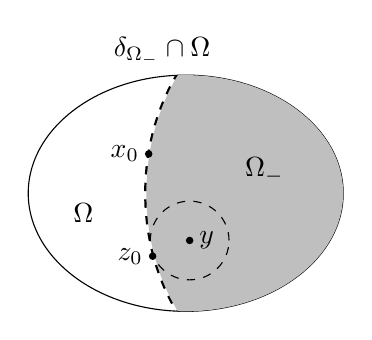
\begin{tikzpicture}
\draw (0,0) ellipse (2cm and 1.5cm);
\begin{scope}
	\clip (0,0) ellipse (2cm and 1.5cm);
	\draw [dashed, ultra thick] (1.5,0) ellipse (2cm and 	2.5cm);
	\path [fill, lightgray] (1.5,0) ellipse (2cm and 2.5cm);
\end{scope}
\draw [fill] (-0.47,0.5) circle [radius=0.4mm] node[left] {$x_0$};
\draw (-0.3,1.5) node[above] 
{$\delta_{\Omega_{-}}\cap \Omega$};
\draw (-1.3,-0.5) node[above] {$\Omega$};
\draw (1,0) node[above] {$\Omega_{-}$};
\draw [dashed] (0.05,-0.6) circle[radius=0.5cm];
\draw [fill] (0.05, -0.6) circle[radius=0.4mm] node[right] {$y$};
\draw [fill] (-0.42, -0.8) circle[radius=0.4mm] node[left] {$z_0$};
\end{tikzpicture}

\caption{$\Omega_{-}\subset\Omega$}
\label{fig:omegamenos}
\end{figure}

\noindent Vamos a tomar un $y\in\Omega$ de tal forma que $y$ esté más cerca de $\delta\Omega_{-}$ que de $\delta\Omega$ y consideramos la bola $B=B(y,R)$ con radio $R$ de tal manera que sea lo mayor posible para que quede dentro de $\Omega_{-}$ (ver figura \ref{fig:omegamenos}).
Llamamos $z_0$ a la intersección de $B$ con $\delta\Omega_{-}$.
Por como está definido $\Omega_{-}$ se puede observar que
$$\delta\Omega_{-}\cap\Omega = \{z\in\Omega: u(z) = u(x_0)\}$$
Así que $u(z_0) = u(x_0) \ge 0$.
Con todo esto, tenemos las hipótesis del \textbf{Lema de Hopf} para $\Omega_{-}$. Utilizando el lema se concluye que
$$\frac{du(z_0)}{d\nu} > 0$$
Como $\frac{du(z_0)}{d\nu} = \nabla u(z_0)\cdot \nu$. Por tanto $$\nabla u(z_0) \cdot \nu > 0\implies \nabla u(z_0) > 0$$
Sin embargo, al ser $u(z_0) = u(x_0)$ un máximo
$$\nabla u(z_0) = 0$$
Tenemos una contradicción al suponer que $u$ tiene un máximo no negativo y que es no constante.
\end{proof}
\newpage
\section{Problemas de condiciones de contorno}
Se denomina problema de condiciones de contorno al conjunto de una ecuación diferencial y datos iniciales en la frontera de una región.

\subsection{Problema de Dirichlet}
El problema de Dirichlet es un problema de valores de contorno que consiste en hallar la solución $u \in C^2(\Omega)\cap C(\overline{\Omega})$ a una EDP en un dominio $\Omega$ acotado de tal forma que:
\begin{equation*}
\text{Si }
\left.
\begin{array}{l}
F\in C(\Omega)\\
f\in C(\delta\Omega)
\end{array}
\right\}
\text{Se quiere hallar } u\text{ tal que }
\left\{
\begin{array}{l r}
\mathcal{L}(u) = F &\text{en } \Omega\\
u = f &\text{en } \Omega\\
\end{array}
\right.
\end{equation*}

\subsubsection{Unicidad}
\begin{prop}{Unicidad del problema de Dirichlet}
Si $\mathcal{L}(u)=\mathcal{L}(v)$ en $\Omega$ y $u=v$ en $\delta\Omega$ entonces $u = v$ en $\Omega$.
\end{prop}
\begin{proof}
Sea $w=u-v$. Como $\mathcal{L}$ es un funcional lineal, se tiene
$$\mathcal{L}(w) = \mathcal{L}(u-v) = \mathcal{L}(u)-\mathcal{L}(v) = 0-0 = 0$$
De las hipótesis se tiene que
\begin{equation*}
\left.
\begin{array}{l l}
\mathcal{L} = 0 & \text{en } \Omega\\
w = 0 & \text{en } \delta\Omega\\
\end{array}
\right\}
\max_{\Omega}w\le\max\{0,\max_{\delta\Omega}w\} = 0
\end{equation*}
es decir, $w\le0$ en $\Omega$. Al ser $\mathcal{L}$ lineal, si $w$ es solución, $-w$ también, por tanto se puede realizar el mismo proceso para llegar a que $-w\le0$ en $\Omega$.
$$w\le0 \wedge -w\le0 \iff w = 0$$
\end{proof}


\subsubsection{Comparación de soluciones}
\begin{prop}{Comparación de soluciones}
Si $\mathcal{L}(u) \le \mathcal{L}(v)$ en $\Omega$ y $u\le v$ en $\delta\Omega$, entonces $u\le v$ en $\Omega$.
\end{prop}
\begin{proof}
Sea $w = u-v$. 
Como $\mathcal{L}$ es un funcional lineal, se tiene
$$\mathcal{L}(w) = \mathcal{L}(u-v) = \mathcal{L}(u)-\mathcal{L}(v) \le 0$$
De las hipótesis se tiene que
\begin{equation*}
\left.
\begin{array}{l l}
\mathcal{L} \le 0 & \text{en } \Omega\\
w \le 0 & \text{en } \delta\Omega\\
\end{array}
\right\}
\max_{\Omega}w\le\max\{0,\max_{\delta\Omega}w\} = 0
\end{equation*}
es decir, $w \le 0$ en $\Omega$. De donde se obtiene que $u\le v$ en $\Omega$.
\end{proof}


\subsection{Problema de Neumann}
El problema de Neumann es un problema de valores de contorno que consiste en hallar la solución $u \in C^2(\Omega)\cap C^1(\overline{\Omega})$ a una EDP en un dominio $\Omega$ acotado de tal forma que:
\begin{equation*}
\text{Si }
\left.
\begin{array}{l}
F\in C(\Omega)\\
f\in C(\delta\Omega)
\end{array}
\right\}
\text{Se quiere hallar } u\text{ tal que }
\left\{
\begin{array}{l r}
\mathcal{L}(u) = F &\text{en } \Omega\\
\frac{du}{d\nu} = f &\text{en } \Omega\\
\end{array}
\right.
\end{equation*}

\subsection{Unicidad}
\begin{prop}{Unicidad del problema de Neumann}
Sean $u,v$ tales que satisfacen $\mathcal{L}(u)=\mathcal{L}(v)$ en $\Omega$ y $\frac{du}{d\nu} = \frac{dv}{d\nu}$ en $\delta\Omega$.
Si $h(x)\ge0$ en $\Omega$ y en todo punto de $\delta\Omega$ se tiene la \textbf{condición de la esfera interior}, entonces $u-v=cte$ en $\Omega$.
\end{prop}
\begin{proof}
Supongamos $w=u-v\neq cte$ en $\Omega$. Al ser $\overline{\Omega}$ un compacto, o bien $w$ o bien $-w$ tiene un máximo no negativo en algún punto $x_0$. Por el principio del máximo, $x_0\in\delta\Omega$.
Por hipótesis se tiene que $\frac{dw(x_0)}{d\nu} = 0$. Sin embargo, por el \textbf{lema de Hopf} $\frac{dw(x_0)}{d\nu} > 0$. Llegamos a una contradicción al suponer que $w=u-v\neq cte$ en $\Omega$.
\end{proof}
\see
\noindent Si $h(x) > 0$ en algún punto de $x\in\Omega$, entonces $u=v$.

\noindent Como $\mathcal{L}(u-v) = 0$, se tiene
$$\mathcal{L}(u-v) = -\Delta (u-v) + \sum_{i=1}^n g_i(x)\frac{d(u-v)}{dx_i} + h(x)(u-v) = 0$$
Pero $u-v=cte$, por lo que queda que
$$h(x)(u-v) = 0$$ Como $h(x)$ es estrictamente positiva, entonces $u-v=0$.

\example
Vamos a ver la necesidad de que $h(x)\ge 0$ en todo el dominio.
Se tiene la ecuación siguiente:
$$-u''-u=0$$
en la que $h(x) = -1 < 0$.
Dos soluciones de esta ecuación son
\begin{equation*}
\begin{array}{l}
u_1(x) = sin(x)\\
u_2(x) = cos(x)\\
\end{array}
\end{equation*}

\begin{figure}[ht]
\centering
\begin{subfigure}{.5\textwidth}
	\centering
  	\begin{tikzpicture}
		\draw[->] (-0.5,0) -- (4,0) node[right] {$x$};
		\draw[->] (0,-1) -- (0,1.5) node[above] {$y$};
		\draw[-] (pi/2,0.1) -- (pi/2,-0.1) node[below] {$\frac{\pi}{2}$};
		\draw[-] (pi,0.1) -- (pi,-0.1) node[below] {$\pi$};
		\draw[] (-0.2,0) node[below] {$0$};
		\draw[fill, blue] (pi/2, 1) circle[radius=0.5mm];
		\draw[scale=1,domain=0:pi,smooth,variable=\x,blue] 
			plot ({\x},{sin(\x r)})
			node[above right] {$u(x)$};
	\end{tikzpicture}
	\caption{$u(x) = sin(x)$}
	\label{fig:sol-contraejemplo-h1}
\end{subfigure}%
\begin{subfigure}{.5\textwidth}
	\centering
  	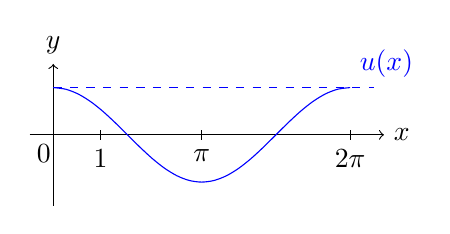
\begin{tikzpicture}[scale=0.6]
		\draw[->] (-0.5,0) -- (7,0) node[right] {$x$};
		\draw[->] (0,-1.5) -- (0,1.5) node[above] {$y$};
		\draw[-] (pi,0.1) -- (pi,-0.1) node[below] {$\pi$};
		\draw[-] (2*pi,0.1) -- (2*pi,-0.1) node[below] {$2\pi$};
		\draw[-, dashed, blue] (0,1) -- (2*pi+0.5,1);
		\draw[] (-0.2,0) node[below] {$0$};
		\draw[-] (1,0.1) -- (1,-0.1) node[below] {$1$};
		\draw[scale=1,domain=0:2*pi,smooth,variable=\x,blue] 
			plot ({\x},{cos(\x r)})
			node[above right] {$u(x)$};
	\end{tikzpicture}
	\caption{$u(x) = cos(x)$}
	\label{fig:sol-contraejemplo-h2}
\end{subfigure}%
\caption{Funciones periódicas}
\label{fig:sol-contraejemplo-h}
\end{figure}

\noindent En la figura \ref{fig:sol-contraejemplo-h1} se puede ver como se alcanza un máximo no negativo en el interior del invervalo. En la figura \ref{fig:sol-contraejemplo-h2} se observa como la función llega a los extremos del intervalo con derivada nula. Ambas situaciones se deben a que no se cumple la condición $h(x) \ge 0$.

\example
Vamos a ver la necesidad de que $\Omega$ sea un dominio acotado.
Sean $u(x,y) = e^xsin(x)$ y $\Omega = \mathbb{R}\times(0, \pi)$
Se tiene que 
\begin{equation*}
u \text{ cumple}
\left\{
\begin{array}{l l}
-\Delta u = 0 & \text{en }\Omega\\
u=0 & \text{en } \delta\Omega\\
\end{array}
\right.
\end{equation*}
\begin{equation*}
\delta\Omega = (\mathbb{R}\times\{0\})\cup(\mathbb{R}\times\{\pi\})
\end{equation*}
Dado que $u(x) = 0$ en toda la frontera, se tiene que cumplir que $u(x) \le 0$ en $\Omega$, sin embargo, esto es falso por no ser $\Omega$ acotado (ver figura \ref{fig:u3d1}).

\begin{figure}[ht]
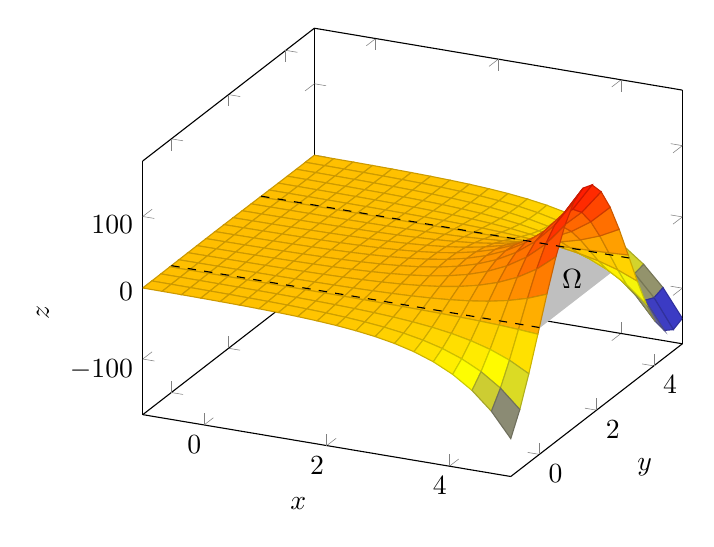
\begin{tikzpicture}
\begin{axis}[
	xlabel=$x$,
	ylabel=$y$,
	zlabel=$z$
]

\addplot3 [color=lightgray, fill] coordinates {(-1,pi,0) (5,pi,0) (5,0,0) (-1,0,0)};

\addplot3[
	surf,
    domain=-1:5,
    samples=20,
	] {(exp(\x))*sin(\y r)};

\addplot3 [color=black, dashed] coordinates {(-1,0,0) (5,0,0)};
\addplot3 [color=black, dashed] coordinates {(-1,pi,0) (5,pi,0)};
\node at (axis cs:4.6,2,0) {$\Omega$};
\end{axis}
\end{tikzpicture}
\caption{$u(x,y) = e^xsin(y)$}
\label{fig:u3d1}
\end{figure}

\newpage
\begin{theorem}
Sea $\Omega$ un dominio acotado, $u\in C^2(\Omega)\cap C(\overline{\Omega})$. 
Sea la inecuación
$$\mathcal{L}(u) \le F  \text{ en } \Omega\\$$
Si $g_1,\hdots,g_n,h$ son acotadas y $h(x) \ge 0$ entonces,
$$u(x) \le \max\{0, \max_{\delta\Omega}u\} + C\max\{0, \max_{\Omega} F\}$$
con $C$ una constante que depende del dominio $\Omega$ y de $g_1,\hdots,g_n$.
\end{theorem}
\begin{proof}
Se va a denotar
\begin{equation*}
\left\{
\begin{array}{l}
\mathcal{L}_0(u)=-\Delta u+\sum_{i=0}^ng_i(x)\frac{du}{dx_i}\\
\mathcal{L}(u) = \mathcal{L}_0(u)+h(x)u\\
M=\max\{0,\max_{\delta\Omega}u\}
\end{array}
\right.
\end{equation*}
Dado que $\Omega$ es un dominio acotado, se tiene que
$\Omega\subset\{x\in\mathbb{R}^n: 0<x_1<d\}$ para algún $d\in\mathbb{R}$.
Definimos $\varphi(x)$ siendo $K$ una constante positiva.
$$\varphi(x)=K\left(e^{\alpha d}-e^{\alpha x_1}\right)+M > M \ge 0$$
Calculamos $\mathcal{L}_0(\varphi)$:
$$\mathcal{L}_0(\varphi)=-Ke^{\alpha x_1}\{-\alpha^2+\alpha \underbrace{g_1(x)}_{\text{acotada}}\}>Ke^{\alpha x_1} > K > 0$$
si tomamos un valor de $\alpha$ lo suficientemente grande.

\noindent Definimos ahora $w=u-\varphi$ y calculamos $\mathcal{L}(w)$:
$$\mathcal{L}(w) = \mathcal{L}(u)-\mathcal{L}(\varphi) \le F - \mathcal{L}_0(\varphi)-\underbrace{h(x)\varphi(x)}_{\ge0}<F(x)-K \le 0$$
Basta tomar $K=\max\{0, \max_{\Omega}F\}$ para tener $\mathcal{L}(w) < 0$.
Por otro lado se tiene que $u\le M$, por tanto $u-\varphi\le M - M = 0$. Es decir, $u \le \varphi$. Entonces 
$$u_\Omega \le \varphi_\Omega\implies u_\Omega \le K\max_\Omega\left(e^{\alpha d}-e^{\alpha x_1}\right) + M = K\left(e^{\alpha d}-1\right) + M$$
\textbf{Conclusión:}

Denotamos $C = \left(e^{\alpha d}-1\right)$. Se puede observar que $C$ depende de $\alpha$ y $d$, es decir, que depende ensencialmente del dominio y de la cota de las funciones $g_1,\hdots,g_n$.
Se tiene entonces que 
$$u(x) \le \max\{0, \max_{\delta\Omega}u\} + C\max\{0, \max_{\Omega} F\}$$
\end{proof}
\newpage
\section{Funciones armónicas}
Esta sección tratará de funciones armónicas. En lo que sigue se denotará con $\Omega$ a un dominio de $\mathbb{R}^n$ y $u$ una función $u$ definida como sigue
$$u:\Omega \in \mathbb{R}^n \longrightarrow \mathbb{R}$$

\begin{definition}{Función armónica}
Se dice que $u$ es \textbf{armónica} $\iff u\in C^2(\Omega)$ y $\Delta u = 0$ en $\Omega$.

\noindent Se dice que $u$ es \textbf{subarmónica} $\iff u\in C^2(\Omega)$ y $\Delta u \ge 0$ en $\Omega$.

\noindent Se dice que $u$ es \textbf{superarmónica} $\iff u\in C^2(\Omega)$ y $\Delta u \le 0$ en $\Omega$.
\end{definition}

\subsection{Propiedad del valor de la media}
\begin{mathresult}{Propiedad de la media de las funciones armónicas}
Sea $u$ una función armónica y $B(x,R)$ una bola de centro $x$ y radio $R$. Si $\overline{B(y,R)}\in \Omega$, se tiene que 
$$u(x) = \frac{1}{|\delta B_R(x)|}\int_{\delta B_R} u(x)dS = \frac{1}{|B_R(x)|} \int_{B_R}u(x)dV$$
donde $\omega_n$ es el área de la bola unidad de dimensión $n$. Es decir, estos tres valores son iguales:
\begin{itemize}
\item El valor de la función en el centro de la bola
\item El valor medio de la función en la superficie de la bola.
\item El valor medio en el interior de la bola.
\end{itemize}

Para funciones \textbf{subarmónicas}, se tiene que el valor en el centro de la bola es \textbf{menor o igual} que el promedio de la función.

Para funciones \textbf{superarmónicas}, se tiene que el valor en el centro de la bola es \textbf{mayor o igual} que el promedio de la función.
\end{mathresult}

\begin{proof}
\indent Sea $u$ una función subarmónica e $y\in\Omega$ un punto del dominio $\Omega$ tal que $\exists B_R(y)$, una bola de radio $R$ centrada en $y$ que cumpe que $\overline{B_R(y)}\in\Omega$.
\vspace{5mm}

En primer lugar vamos a definir $\omega_n$ como el área de la superficie bola unitaria de dimensión $n$. Es decir
$$\omega_n = \frac{2\pi^{n/2}}{\Gamma(n/2)}$$ De esta manera, el volumen de la misma bola será $\omega_n/n$.
Realizando un simple cambio de variable, se obtiene que el área de la superficie de la bola de radio $R$ de dimensión $n$ es $\omega_nR^{n-1}$ y su volumen $\frac{R^n\omega_n}{n}$.

En resumen:
\begin{equation*}
\left\{
\begin{array}{l}
\text{Área}(\delta B_1) = \omega_n\\
\text{Vol}(B_1) = \frac{\omega_n}{n}\\
\text{Área}(\delta B_R) = \omega_nR^{n-1}\\
\text{Vol}(B_R) = \frac{R^n\omega_n}{n}
\end{array}
\right.
\end{equation*}

Consideramos
$$g(\rho) = \frac{1}{|\delta B_\rho|}\int_{\delta B_\rho(y)} u(\xi)dS_\xi = \frac{1}{\omega_n \rho^{n-1}}\int_{\delta B_\rho(y)} u(\xi)dS_\xi$$ para un $\rho \in (0,R)$.

Realizamos ahora un cambio de variable para llevar el resultado a la bola unidad.
\begin{equation*}
\left\{
\begin{array}{l}
\xi = y+\rho w\\
w = \frac{\xi-y}{\rho}\\
|w| = 1
\end{array}
\right.
\end{equation*}
Se tiene
$$g(\rho) = \frac{1}{\omega_n \rho^{n-1}}\int_{\delta B_\rho(y)} u(\xi)dS_\xi = \frac{\rho^{n-1}}{\omega_n \rho^{n-1}}\int_{\delta B_1(y)} u(y+\rho w)dS_w$$
Tomamos ahora 
$$g'(\rho) = \frac{1}{\omega_n}\int_{\delta B_1(y)} \nabla u(y+\rho w)wdS_w$$
Definimos $v(y)$ de forma que cumpla:
\begin{equation*}
\left\{
\begin{array}{l}
v(w) = u(y+\rho w)\\
\nabla v(w) = \nabla u(y+\rho w)\rho\\
\Delta v(y) = \rho^2\Delta u(y+\rho w)
\end{array}
\right.
\end{equation*}
por tanto 
$$g'(\rho) =  \frac{1}{\omega_n}\int_{\delta B_1(y)} \frac{1}{\rho} \nabla v(w)wdS_w =  \frac{1}{\omega_n \rho}\int_{\delta B_1(y)} <\nabla v(w), w>dS_w$$
usando el teorema de la divergencia
$$g'(\rho) =  \frac{1}{\omega_n \rho}\int_{B_1(y)} \Delta v(w)dS_w = 0$$
Si $g'(\rho) = 0\implies g(\rho) = cte$ en $(0,R)$. Como $u$ es continua, $g(\rho) = u(y)$.

$$u(y) = \frac{1}{|\delta B_\rho(y)|}\int_{\delta B_\rho(y)}u(\xi)dS_\xi$$
lo que ocurre $\forall \rho \in (0,R)$

Por otro lado, si lo anterior se integra en $(0,R)$
$$\int_0^R u(y) d\rho = \frac{R^n}{n}u(y) = \frac{1}{\omega_n} \int_0^R d\rho \int_{\delta B_\rho(y)} u (\xi) dS_\xi = \frac{1}{\omega_n}\int_{B_R(y)} u(x) dx$$
Luego 
$$u(y) = \frac{n}{\omega_n R^n}\int_{B_R(y)} u(x) dx = \frac{1}{|B_R(y)|} \int_{B_R(y)} u(x) dx$$
\end{proof}


\begin{mathresult}{Principio fuerte del máximo para funciones subarmónicas}
Sea $u(x)$ una función armónica en $\Omega$. Si $u$ alcanza su máximo en $\Omega$, entonces $u$ es constante en $\Omega$.
\end{mathresult}
\begin{proof}
Sea $M=\sup_\Omega u$ y $\Omega_M = \{x\in\Omega: u(x) = M\}$. Está claro que $\Omega_M$ es cerrado relativo a $\Omega$. Vamos a demostrar que $\Omega_M$ es también un abierto relativo a $\Omega$. De esta forma, como $\Omega$ es un dominio, al ser conexo, los únicos subconjuntos que son simultáneamente abiertos y cerrados son el vacío y el propio $\Omega$. Si $u$ tiene un máximo en $x_0$, tendríamos que $x_0\in\Omega_M\neq\emptyset$. Luego, $\Omega_M = \Omega$.

Sea $z\in\Omega_M$. Tenemos
$$0=(u(z) - M) = \frac{1}{|B_R|}\int_{B_R}(u(x)-M)dx = \frac{1}{|B_R|}\int_{B_R} 0dx = 0$$
Es decir, tenemos que $u(x)-M = 0$ en toda la bola. Por lo que para todo $z\in\Omega_M$ podemos encontrar una bola $B$ abierta tal que $B\in\Omega_M$, luego $\Omega_M$ es abierto.
\end{proof}

\subsection{Solución del problema de Dirichlet para el disco unidad}
\noindent De aquí en adelante, se denotará
$$\mathbb{D} = \{(x,y)\in \mathbb{R}^2: x^2+y^2 < 1\}$$
Dada $f\in\delta\mathbb{D}$, continua, $2\pi-$periódica y definida como sigue:
$$f:\mathbb{R}\longrightarrow\mathbb{R}$$
se quiere encontrar $u\in C^2(\mathbb{D})\cap C(\mathbb{\overline{\mathbb{D}}})$ que satisfaga
\begin{equation*}
\left\{
\begin{array}{l l}
-\Delta u = 0 & \text{en } \mathbb{D}\\
u=f & \text{en } \delta\mathbb{D}
\end{array}
\right.
\end{equation*}
Las soluciones que buscamos tienen la forma
$$u(x,y) = R(r)T(\theta)$$
con $r=||(x,y)||=\sqrt{x^2+y^2}$
Dado que la función $u$, es armónica, $u$ verifica $\Delta u = 0$, o lo que es lo mismo
$$R''T+\frac{1}{r}R'T+\frac{1}{r^2}RT'' = 0$$
Separando las variables, se obtiene
$$\frac{r^2R''+rR'}{R}=\frac{-T''}{T}$$
Observamos que tenemos una igualdad de dos funciones que dependen de variables distintas. El primer término depende sólamente de $r$, mientras que el segundo depende de $\theta$. Esto implica que dichos términos han de ser iguales a una constante $\lambda$, luego se tiene que
\begin{align}\label{eq:dirich1}
r^2R''+rR'-\lambda r = 0\\\label{eq:dirich2}
T''+\lambda T = 0
\end{align}
Tenemos un sistema de dos EDOs independientes, la primera es la ecuación de Cauchy-Euler, y la segunda es sencilla de resolver.
Las posibles soluciones para ambas EDOs son:
\begin{equation*}
\eqref{eq:dirich1}\ R(r) = \left\{
\begin{array}{l l}
1,log(r) & \lambda=0\\
r^{\sqrt{\lambda}}, r^{-\sqrt{\lambda}} & \lambda > 0\\
\text{soluciones complejas} & \lambda < 0
\end{array}
\right.
\end{equation*}
\begin{equation*}
\eqref{eq:dirich2}\ T(\theta) = \left\{
\begin{array}{l l}
1,\theta & \lambda=0\\
cos(\sqrt{\lambda}\theta), sin(\sqrt{\lambda}\theta) & \lambda > 0\\
cosh(\sqrt{-\lambda\theta}), sinh(\sqrt{-\lambda\theta}) & \lambda < 0
\end{array}
\right.
\end{equation*}
No se puede suponer que para todos los valores de $\lambda$ y para toda elección de $R$ y $T$, la fórmula $u(x,y) = R(r)T(\theta)$ va a definir una función armónica en un dominio $\Omega$. Esto es sólo verdad si se define una función $C^2(\Omega)$. Si $\Omega$ contiene curvas que encierran al origen, entonces la función $u$ será $2\pi-$periódica. En este caso $\Omega=\mathbb{D}$, por lo que $u$ ha de ser $2\pi-$periódica.

\noindent Eliminamos las siguientes soluciones por no ser $2\pi-$periódicas.
\begin{equation*}
\eqref{eq:dirich2}\ T(\theta) = \left\{
\begin{array}{l l}
1,\color{red}{\theta} & \lambda=0\\
cos(\sqrt{\lambda}\theta), sin(\sqrt{\lambda}\theta) & \lambda > 0\\
\color{red}{cosh(\sqrt{-\lambda\theta})}, \color{red}{sinh(\sqrt{-\lambda\theta})} & \lambda < 0
\end{array}
\right.
\end{equation*}
Para que
\begin{equation*}
\left.
\begin{array}{l l}
cos(\sqrt{\lambda}(\theta+2\pi)) = cos(\sqrt{\lambda}(\theta))\\
sin(\sqrt{\lambda}(\theta+2\pi)) = sin(\sqrt{\lambda}(\theta))\\
\end{array}
\right\} \iff \lambda = n^2
\end{equation*}
con $n=1,2,3,\hdots$

\noindent Eliminamos las siguientes soluciones dado que $(0,0)\in\mathbb{D}$
\begin{equation*}
\eqref{eq:dirich1}\ R(r) = \left\{
\begin{array}{l l}
1,\color{red}{log(r)} & \lambda=0\\
r^{\sqrt{\lambda}}, \color{red}{r^{-\sqrt{\lambda}}} & \lambda > 0\\
\end{array}
\right.
\end{equation*}
Se tiene entonces que $u$ es combinación lineal de las soluciones anteriores (tomamos la constante como $\frac{a_0}{2}$ por comodidad):
$$u_N(x,y) = \frac{a_0}{2}+\sum_{n=1}^Nr^n(a_ncos(n\theta)+b_nsin(n\theta))$$
La condición de frontera del problema de Dirichlet pide que $u=f$ en $\delta\Omega$. Por tanto
$$U_N(1,\theta) = f(\theta)$$
Si $f$ se puede escribir como combinación lineal de senos y cosenos, entonces el problema tiene solución y como ya se ha visto, dicha solución es única.
Supongamos que
$$f(\theta) = \frac{a_0}{2} + \sum_{n=1}^\infty (a_ncos(n\theta)+b_nsin(n\theta))$$
Se puede observar (ver figura \ref{fig:int-period}) que
\begin{equation*}
\int_0^{2\pi} cos(n\theta)d\theta = \int_0^{2\pi} sin(n\theta)d\theta=0
\end{equation*}
\begin{figure}[ht]
	\centering
	\begin{subfigure}{.5\textwidth}
	\centering
	\begin{tikzpicture}
	    \fill[fill=lavenderblue, samples=400, scale=0.5] (0,0) -- plot [domain=0:2*pi] (\x,{sin(4*(\x r))}) -- (2*pi,0) -- cycle;
    	\draw plot[domain=0:2*pi, samples=400, scale=0.5] (\x,{sin(4*(\x r))});
	    \draw[->] (-0.3,0) -- (pi+0.3,0);
	    \draw[->] (0,-0.3) -- (0,1.3);
	\end{tikzpicture}
	\caption{$sin(n\theta)$}
	\end{subfigure}%
	%
	\begin{subfigure}{.5\textwidth}
	\centering
	\begin{tikzpicture}
	    \fill[fill=lavenderblue, samples=400, scale=0.5] (0,0) -- plot [domain=0:2*pi] (\x,{cos(4*(\x r))}) -- (2*pi,0) -- cycle;
    	\draw plot[domain=0:2*pi, samples=400, scale=0.5] (\x,{cos(4*(\x r))});
	    \draw[->] (-0.3,0) -- (pi+0.3,0);
	    \draw[->] (0,-0.3) -- (0,1.3);
	\end{tikzpicture}
	\caption{$cos(n\theta)$}
	\end{subfigure}
	\caption{Integrales periódicas}
	\label{fig:int-period}
\end{figure}
Luego
$$\int_0^{2\pi} f(\theta)d\theta = \frac{a_0}{2}2\pi+0$$
obteniéndose así
$$\frac{a_0}{2} = \frac{1}{2\pi}\int_0^{\pi}f(\theta)d\theta$$
Ahora vamos a ver los valores que toman $a_n$ y $b_n$ para cada valor de $n$.
\begin{itemize}
\item Valor de $a_n$
\begin{align*}
\int_0^{2\pi}f(\theta)cos(m\theta)d\theta = & \frac{a_0}{2}\underbrace{\int_0^{2\pi}cos(m\theta)}_{=0} +\\
+ & \sum_{n=1}^\infty\left(a_n\underbrace{\int_0^{2\pi}cos(n\theta)cos(m\theta)d\theta}_{=\pi}\right) +\\
+ & \sum_{n=1}^\infty\left(b_n\underbrace{\int_0^{2\pi}sin(n\theta)cos(m\theta)d\theta}_{=0}\right)
\end{align*}
Luego
$$a_m = \frac{1}{\pi}\int_0^{2\pi}f(\theta)cos(m\theta)d\theta$$
\item Valor de $b_n$
\begin{align*}
\int_0^{2\pi}f(\theta)sin(m\theta)d\theta = & \frac{a_0}{2}\underbrace{\int_0^{2\pi}sin(m\theta)}_{=0} +\\
+ & \sum_{n=1}^\infty\left(a_n\underbrace{\int_0^{2\pi}cos(n\theta)sin(m\theta)d\theta}_{=0}\right) +\\
+ & \sum_{n=1}^\infty\left(b_n\underbrace{\int_0^{2\pi}sin(n\theta)sin(m\theta)d\theta}_{=\pi}\right)
\end{align*}
Luego
$$b_m = \frac{1}{\pi}\int_0^{2\pi}f(\theta)sin(m\theta)d\theta$$
\end{itemize}
Tenemos entonces que $u$ es de la forma
\begin{align*}
u(r,\theta) = & \frac{a_0}{2}+\sum_{n=1}^\infty r^n\left(a_ncos(n\theta)+b_n sin(n\theta)\right) =\\
= & \frac{1}{2\pi}\int_0^{2\pi}f(\theta)d\theta+\\
+ & \sum_{n=1}^\infty r^n\left(\frac{1}{\pi}\int_0^{2\pi}f(\varphi)cos(n\varphi)d\varphi cos(n\theta)\right) + \\
+ & \sum_{n=1}^\infty r^n\left(\frac{1}{\pi}\int_0^{2\pi}f(\varphi)sin(n\varphi)d\varphi sin(n\theta)\right) = \\
= & \frac{1}{\pi}\int_0^{2\pi}f(\varphi)\left\{\frac{1}{2}+\sum_{n=1}^\infty r^n\left(cos(n\varphi)cos(n\theta)+sin(n\varphi)sin(n\theta)\right)\right\}d\varphi = \\
= & \frac{1}{\pi}\int_0^{2\pi}f(\varphi)\left\{\frac{1}{2}+\sum_{n=1}^\infty r^n\left(cos(n(\theta-\varphi))\right)\right\}d\varphi 
\end{align*}
En definitiva:
$$u(r,\theta) = \int_0^{2\pi}f(\varphi)P(r,\theta-\varphi)d\varphi$$
donde
$$P(r,\varphi)=\frac{1}{\pi}\left\{\frac{1}{2}+\sum_{n=1}^\infty r^n cos(n\varphi)\right\}$$
Vamos a calcular el valor de $P(r, \varphi)$. Sea $z=re^{i\varphi}$. Se tiene que $z^n=r^ne^{in\varphi}$. Si $|z|<1$, se tiene que
$$\sum_{n=1}^\infty z^n = \frac{z}{1-z}$$
Así que 
$$\sum_{n=1}^\infty z^n + \frac{1}{2} = \frac{1+z}{2(1-z)}$$
Entonces
$$P(r,\varphi) = \frac{1}{2\pi}Re\left(\frac{1+z}{1-z}\right)$$
Vamos a simplificar este valor, multiplicando el numerador y el denominador por el conjugado de $1-z$.
$$\frac{1+z}{1-z}\cdot\frac{1-\overline{z}}{1-\overline{z}} = \frac{1-r^2+(z-\overline{z})}{|1-\overline{z}|^2} = \frac{1-r^2-2iIm(z)}{1+r^2-2Re(z)}$$
De donde se obtiene la parte real de $\frac{1+z}{1-z}$
$$P(r,\varphi) = \frac{1}{2\pi}\cdot\frac{1-r^2}{1-2rcos(\varphi)+r^2}$$
\begin{mathresult}{Solución del problema de Dirichlet}
La solución del problema de Dirichlet en el disco unidad es de la forma $$u(r,\theta) = \int_0^{2\pi}f(\varphi)P(r,\theta-\varphi)d\varphi$$
donde $P(r, \varphi)$ es el núcleo de Poisson.
$$P(r,\varphi) = \frac{1}{2\pi}\cdot\frac{1-r^2}{1-2rcos(\varphi)+r^2}$$
\end{mathresult}
\subsubsection{Núcleo de Poisson}
Como ya se ha visto, el \textbf{núcleo de Poisson} tiene la forma $$P(r,\varphi) = \frac{1}{2\pi}\cdot\frac{1-r^2}{1-2rcos(\varphi)+r^2}$$
Veamos unas pocas propiedades de esta función
\begin{itemize}
\item \textbf{Definición}

\begin{equation*}
\text{El núcleo de Poisson está definido en}
\left\{
\begin{array}{l}
0\le r\le 1\\
\varphi \neq 0
\end{array}
\right.
\text{ver figura \ref{fig:def-poisson}.}
\end{equation*}

\begin{figure}[ht]
\centering
\begin{tikzpicture}[scale=1.5]
	\draw[->] (-1.5,0) -- (1.5,0) node[right] {$x$};
	\draw[->] (0,-1.5) -- (0,1.5) node[above] {$y$};
	\draw [fill, lavenderblue] (0,0) circle [radius=1];
	\draw [] (0,0) circle [radius=1];
	\draw [fill, white] (1,0) circle [radius=0.07];
	\draw [] (1,0) circle [radius=0.07];
	\node (0,0) {$\mathbb{D}$};
\end{tikzpicture}
\caption{Dominio del núcleo de Poisson}
\label{fig:def-poisson}
\end{figure}

\item $P(r, \varphi)$ \textbf{es armónica}
Dado que $u(r,\theta)$ es armónica y 
$$u(r,\theta)=\int_0^{2\pi}f(\varphi)P(r,\theta-\varphi)d\varphi$$
Se tiene que 
$$0 = \Delta u(r,\theta)=\int_0^{2\pi}f(\varphi)\Delta P(r,\theta-\varphi)d\varphi$$
Es decir
$$\Delta P(r,\theta) = 0$$

\item $\int_0^{2\pi}P(r,\varphi)d\varphi = 1$

Basta tomar $f(\theta) = 1$ y comprobar que $u=1$ es solución. Por tanto
$$u(r, \theta) = 1 = \int_0^{2\pi}1\cdot P(r,\theta-\varphi)d\varphi$$

\item $\int_{-\pi}^{\pi}P(r,\varphi)d\varphi = 1$

Dado que las integrales necesarias para calcular lo anterior tienen el mismo valor entre $-\pi$ y $\pi$, basta repetir la prueba anterior.
\end{itemize}

\begin{theorem}

Si $f$ es continua en $\theta_0$, entonces
$$\lim_{(r,\theta)\to(1,\theta_0)}=f(\theta_0)$$
\end{theorem}
\begin{proof}
Vamos a calcular
$$u(r,\theta)-f(\theta_0)$$
Dado que $$\int_{-\pi}^{\pi}P(r,\tilde{\varphi})d\tilde{\varphi} = 1$$
Se tiene que 
$$u(r,\theta)-f(\theta_0)\cdot 1 = u(r,\theta)-f(\theta_0)\int_{-\pi}^{\pi}P(r,\tilde{\varphi})d\tilde{\varphi}$$
Si realizamos el siguiente cambio de variable:
\begin{equation*}
\left.
\begin{array}{l}
\tilde{\varphi} = \theta+\varphi\\
d\tilde{\varphi} = d\varphi
\end{array}
\right\}
\end{equation*}
entonces
$$u(r,\theta)-f(\theta_0)\int_{-\pi}^{\pi}P(r,\tilde{\varphi})d\tilde{\varphi}=\frac{1-r^2}{2\pi}\int_{-\pi}^{\pi}\frac{f(\theta_0+\varphi)-f(\theta_0)}{1-2rcos(\theta-\theta_0-\varphi)+r^2}$$
Podemos separar lo anterior en tres integrales
$$u(r,\theta)-f(\theta_0)=\frac{1-r^2}{2\pi}\left(\int_{-\pi}^{-\delta}\int_{-\delta}^{\delta}\int_{\delta}^{\pi}\right)\left(\frac{f(\theta_0+\varphi)-f(\theta_0)}{1-2rcos(\theta-\theta_0-\varphi)+r^2}\right)$$
La continuidad de $f$ nos dice que dado un $\varepsilon>0, \exists\delta$ tal que
$$|\varphi|<\delta \implies |f(\theta+\varphi)-f(\theta_0)| < \frac{\varepsilon}{2}$$
Vamos a calcular la integral del medio:
\begin{align*}
\frac{1-r^2}{2\pi}\int_{-\delta}^{\delta}\left(\frac{f(\theta_0+\varphi)-f(\theta_0)}{1-2rcos(\theta-\theta_0-\varphi)+r^2}\right) & \le \\
\frac{1-r^2}{2\pi}\int_{-\delta}^{\delta}\left(\frac{\varepsilon/2}{1-2rcos(\theta-\theta_0-\varphi)+r^2}\right) & =
\frac{\varepsilon}{2}\int_{-\delta}^{\delta}\left(P(r,\varphi)d\varphi\right) = \frac{\varepsilon}{2}\\
\end{align*}
Manteniendo el valor de $\delta$ fijo, si $|\varphi| > \delta$ y $|\theta-\theta_0|<\frac{\delta}{2}$, se tiene que
$$|\theta-\theta_0-\varphi| \ge |\varphi|-|\theta-\theta_0|>\delta-\frac{\delta}{2} = \frac{\delta}{2}$$
Calculamos las otras dos integrales, tomando $M=\max_{\delta\mathbb{D}}f$
\begin{align*}
\frac{1-r^2}{2\pi}\left(\int_{-\pi}^{-\delta}\int_{-\delta}^{\delta}\int_{\delta}^{\pi}\right)\left(\frac{f(\theta_0+\varphi)-f(\theta_0)}{1-2rcos(\theta-\theta_0-\varphi)+r^2}\right)\le \\
\le \frac{2M}{2\pi}\cdot\frac{1-r^2}{1-2rcos(\theta-\theta_0-\varphi)+r^2}\cdot 2(\pi-\delta)\to 0
\end{align*}
si $r\to 1$.
Tenemos por tanto que
$$u(r,\theta)-f(\theta_0) \le \frac{\varepsilon}{2} + \frac{\varepsilon}{2} = \varepsilon$$
\end{proof}

\subsection{Fórmula de representación}
Vamos a buscar soluciones radiales para $\Delta u = 0$ en $\mathbb{R}^n$, lo que quiere decir que buscamos $f(r)$ tal que
$$u(x) = f(r)$$ con $r=||x||$

En primer lugar vamos a hallar el laplaciano en función de $r$.

\begin{equation*}
\begin{array}{l l l}
\frac{du(x)}{dx_i} & = & f'(r)\frac{x_i}{r}\\
\frac{d^2u(x)}{dx_i^2} & = & f''(r)\frac{x_i^2}{r^2}+f'(r)\frac{r^2-x_i\frac{x_i}{r}}{r^2}\\
& = & f''(r)\frac{x_i^2}{r^2}+f'(r)\frac{r^2-x_i^2}{r^3}\\
\Delta u(x) & = & \sum_{i=0}^N\frac{d^2u(x)}{dx_i^2} = f''(r)+f'(r)\frac{N-1}{r} = \frac{1}{r^{N-1}}\left(r^{N-1}f'(r)\right)'
\end{array}
\end{equation*}

Vamos a calcular soluciones radiales para
\begin{equation*}
\left\{
\begin{array}{l l}
\Delta u(x) = 0 & \text{en } \mathbb{R}^n\\
u(x) = f(r)
\end{array}
\right.
\end{equation*}
Como $\Delta u(x) = \frac{1}{r^{N-1}}\left(r^{N-1}f'(r)\right)'$ y $\Delta u(x) = 0$. Se tiene que $\left(r^{N-1}f'(r)\right)$ es constante
$$r^{N-1}f'(r) = A$$ de donde se obtiene
$$f(r) = \frac{A}{N-2}\cdot \frac{1}{r^{N-2}} + B$$ con $A,B$ constantes.

Si $u(x) = 1$, tenemos que la solución es 
$\Gamma(x) = \frac{1}{r^{N-2}} = \frac{1}{||x||^{N-2}}$ para $N\neq 2$ y $\Gamma(x) = log(r)$ para $N=2$. En cualquier caso se cumple que $\Delta\Gamma(x) = 0$ en $\mathbb{R}^N\setminus\{ 0 \}$

En lo que sigue vamos a tener presente las siguientes equivalencias
\begin{equation*}
\begin{array}{l}
\Delta u = div \nabla u = \nabla^2 u\\
div(f\cdot F) = f\cdot div(F)+div(f)\cdot F
\end{array}
\end{equation*}
De esta forma, se cumplen las igualdades que siguen:
\begin{equation*}
\left\{
\begin{array}{l}
div(v\nabla u)=v\Delta u+\nabla v\nabla u\\
div(u\nabla v)=u\delta v+\nabla u\nabla v\\
\end{array}
\right.
div(v\nabla u-u\nabla v) = v\Delta u-u\Delta v
\end{equation*}
Sea $y\in \Omega$ un punto tal que $\exists B_\varepsilon(y)$, una bola $B$ de radio $\varepsilon$ que cumple $\overline{B_\varepsilon(y)}\in\Omega$. Definimos
$$\Omega_\varepsilon = \Omega\setminus \overline{B_\varepsilon(y)}$$
Consideramos ahora 
$$\int_{\Omega_\varepsilon} \left(v\Delta u-u\Delta v\right)dx =\int_{\Omega_\varepsilon} div\left(v\nabla u-u\nabla v\right)dx $$
Utilizando el teorema de la divergencia
$$\int_{\Omega_\varepsilon} div\left(v\nabla u-u\nabla v\right)dx =\int_{\delta\Omega_\varepsilon} \left(v\frac{du}{d\nu}-u\frac{dv}{d\nu}\right)d\xi$$
con $\nu$ la normal exterior a $\delta\Omega_\varepsilon$.

Tomamos $v(x) = \Gamma(x-y)$ que como ya hemos visto cumple que $\Delta v(x) = 0$ en $\mathbb{R}^N\setminus\{y\}$.

Utilizando el resultado anterior y que $\delta \Omega_\varepsilon = \delta\Omega \cup \delta B_\varepsilon(y)$ 
\begin{align*}
& \int_{\Omega_\varepsilon} \frac{1}{|x-y|^{N-2}}\Delta u(x)dx =\\
& \int_{\delta\Omega_\varepsilon} \left(\frac{1}{|\xi-y|^{N-2}}\frac{du(\xi)}{d\nu}-u(\xi)\frac{d}{d\nu}\left(\frac{1}{|\xi-y|^{N-2}}\right)\right)dS_\xi \ + \\
& \int_{\delta B_\varepsilon(y)} \left(\frac{1}{\varepsilon^{N-2}}\frac{du(\xi)}{d\nu}-u(\xi)\frac{d}{d\nu}\left(\frac{1}{|\xi-y|^{N-2}}\right)\right)dS_\xi\\
\end{align*}

Vamos a estudiar ambos términos por separado. Sea $M=\max_{\overline{\Omega}}|\nabla u(x)|$, como $u\in C^2(\Omega)\cup C^1(\overline{\Omega})$, si $\varepsilon\to 0$
\begin{align*}
& \int_{\delta B_\varepsilon(y)} \left(\frac{1}{\varepsilon^{N-2}}\frac{du(\xi)}{d\nu}-u(\xi)\frac{d}{d\nu}\left(\frac{1}{|\xi-y|^{N-2}}\right)\right)dS_\xi \ \le\\
& \frac{1}{\varepsilon}M\int_{\delta B_\varepsilon(y)} dS_\varepsilon \ = \frac{1}{\varepsilon^{N-2}}M|\delta B_\varepsilon| \ = M\omega_n\varepsilon\to 0\\
\end{align*}

En $\delta B_\varepsilon$ tenemos que $\nu = \frac{\xi-y}{\varepsilon}$ por tanto, si $\varepsilon\to0$
$$\frac{d}{d\nu}\left(\frac{1}{|\xi-y|^{N-2}}\right) = -\left.\frac{d}{dr}\right|_{r=\varepsilon}\frac{1}{r^{N-2}} = (N-2)\varepsilon^{1-N}$$ si tomamos $r=|\xi-y|$. Luego
\begin{align*}
& \int_{\delta B_\varepsilon} u(\xi)\frac{d}{d\nu}\left(\frac{1}{|\xi-y|^{N-2}}\right)dS_\xi \ = (N-2)\varepsilon^{1-N}\int_{\delta B_\varepsilon}u(\xi)dS_\xi \ = \\
& (N-2)\varepsilon^{1-N}\varepsilon^{N-1}\int_{\delta B_1}u(y+\varepsilon w)dS_\xi\to(N-2)|\delta B_1|u(y)
\end{align*}

Nos queda que 
\begin{align*}
|N-2||\delta B_1|u(y) = & -\int_{\Omega}\frac{\Delta u(x)}{|x-y|^{N-2}}dx\\
& + \int_{\delta\Omega} \frac{1}{|\xi-y|^{N-2}}\cdot\frac{du(\xi)}{d\nu}dS_\xi\\
& -\int_{\delta\Omega}u(\xi)\frac{d}{d\nu}\left(\frac{1}{|\xi-y|^{N-2}}\right)dS_\xi
\end{align*}

Esta fórmula de representación implica que
\begin{equation*}
\left.
\begin{array}{l l}
\Delta u & \text{en } \Omega\\
u & \text{en } \delta\Omega\\
\frac{du}{d\nu} & \text{en } \delta\Omega\\
\end{array}
\right\} \text{determinan } u \text{ en } \Omega
\end{equation*}
Se necesitan conocer tres valores, mientras que en el problema de Dirichlet sólo hemos necesitado los dos primeros. Por ello, vamos a manipular la fórmula para que deje de depender del tercer término. Sea $h(x)$ una función armónica. El teorema de la divergencia dice que
$$\int_{\Omega}h(x)-\Delta u(x) - u(x)\Delta h(x) = \int_{\delta\Omega}\left(h\frac{du}{d\nu}-u\frac{dh}{d\nu}\right)$$
Luego 
$$\int_{\Omega}h(x)-\Delta u(x) - u(x)\Delta h(x) - \int_{\delta\Omega}\left(h\frac{du}{d\nu}-u\frac{dh}{d\nu}\right) = 0$$
Sumar esta diferencia a la fórmula de representación que ya tenemos es como sumarle 0. Por simplicidad de notación, vamos a denotar $G(x,y) = \frac{1}{|x-y|^{N-2}}+h(x)$. Tras realizar la suma:
\begin{align*}
|N-2||\delta B_1|u(y) = & -\int_{\Omega}G(x,y)\Delta u(x)dx\\
& + \int_{\delta\Omega} G(\xi, y)\frac{du(\xi)}{d\nu}dS_\xi\\
& -\int_{\delta\Omega}u(\xi)\frac{dG(\xi, y)}{d\nu}dS_\xi
\end{align*}
Queremos librarnos del segundo término, por lo que hay que elegir $h$ para que $G$\footnote{$G$ se conoce como la función de Green para el dominio $\Omega$} sea $0$ en la frontera de $\Omega$. Tomamos $h(x) = \frac{1}{|\xi-y|^{N-2}}$ con $\xi\in\delta\Omega$. Se cumple que $\Delta G(x,y) = 0 \ \forall x \in R^N\setminus \{y\}$ y que $G(\xi,y) = 0 \ \forall \xi \in \delta \Omega$. Tenemos un problema de Dirichlet en $\Omega\setminus\{y\}$.

\subsection{Núcleo de Poisson N-dimensional}
El núcleo de Poisson $N-$dimensional es la función de Green para el dominio $\Omega=B_r(0)$.
Supongamos que $\Delta u = 0$ en $B_r(0)$, y fijemos $x\in B_r(0)$
La fórmula de representación queda de esta forma:
\begin{align*}
|N-2||\delta B_1|u(x) = & -\int_{\Omega}\overbrace{\frac{\Delta u(x)}{|x-y|^{N-2}}}^{0}dx\\
& + \int_{\delta\Omega} \frac{1}{|\xi-x|^{N-2}}\cdot\frac{du(\xi)}{d\nu}dS_\xi\numberthis\label{eq:repr-dirichlet-formula}\\
& -\int_{\delta\Omega}u(\xi)\frac{d}{d\nu}\left(\frac{1}{|\xi-x|^{N-2}}\right)dS_\xi
\end{align*}
Vamos a definir $x'$ como el simétrico de $x$ respecto de la bola. Dada esta definición de $x'$, tenemos que cumple:
\begin{equation*}
\begin{array}{l}
|x||x'|=R^2\\
x'=\frac{R^2}{|x|^2}x
\end{array}
\end{equation*}
Ahora consideramos
$$v(y) = \frac{1}{|y-x'|^{N-2}}$$ que está definida en $\mathbb{R}^N\setminus\{x\}$ y cumple $\Delta v(y) = 0$ en todo su dominio de definición.
Se tiene que
$$\int_\Omega v\underbrace{\Delta u}_0 -u\underbrace{\Delta v}_0 = \int_{\delta B_r} \left(v\frac{du}{d\nu}-u\frac{dv}{d\nu}\right)dS = 0$$
\begin{figure}[ht]
\centering
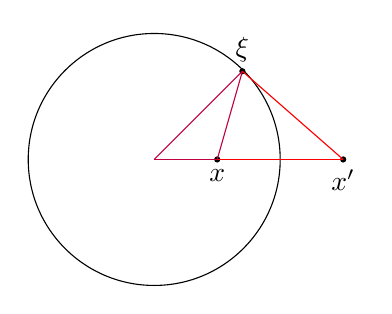
\begin{tikzpicture}[scale=1.6]
\draw[] (0,0) circle[radius=1];
\draw[fill] (0.5,0) circle[radius=0.02] node[below] {$x$};
\draw[fill] (1.5,0) circle[radius=0.02] node[below] {$x'$};
\draw[fill] (0.7,0.7) circle[radius=0.02] node[above] {$\xi$};
\draw[-, purple] (0,0)--(0.5,0);
\draw[-, red] (0.5,0)--(1.5,0);
\draw[-, purple] (0,0)--(0.7,0.7);
\draw[-, purple] (0.5,0)--(0.7,0.7);
\draw[-, red] (1.5,0)--(0.7,0.7);
\end{tikzpicture}
\caption{Dominio $B_r(0)$}
\label{fig: dominiobr}
\end{figure}

Los triángulos $0x\xi$ y $0x'\xi$ son semejantes (ver figura \ref{fig: dominiobr}). Se tiene que
$$\frac{|x|}{R} = \frac{R}{|x'|}$$ Luego $$\frac{|x-\xi|}{|x|} = \frac{|\xi-x'|}{R}$$ es decir, el resto de lados respetan la relación. Todo esto es lo mismo que
$$\frac{1}{|\xi-x|} = \frac{R}{|x|}\cdot\frac{1}{|\xi-x'|}$$
Ya hemos visto que
$$A = \int_{\delta B_r} \left(v\frac{du}{d\nu}-u\frac{dv}{d\nu}\right)dS = 0$$
De donde también se tiene que
$$0 = \left(\frac{R}{|x|}\right)A$$
Luego si a \eqref{eq:repr-dirichlet-formula} le restamos $\left(\frac{R}{|x|}\right)A$ es como si le restáramos $0$.
Nos queda lo siguiente
\begin{align*}
|N-2||\delta B_1|u(x) = \int_{\delta B_r}\left(\overbrace{\frac{1}{|\xi-x|^{N-2}}-\left(\frac{R}{|x|}\right)^{N-2}\frac{1}{|\xi-x'|^{N-2}}}^0\right)\frac{du}{d\nu}dS\\
+ \int_{\delta B_r}u(\xi)\left(\left(\frac{R}{|x|}\right)^{N-2}\frac{d}{d\nu}\left(\frac{1}{|\xi-x'|^{N-2}}\right)-\frac{d}{d\nu}\left(\frac{1}{|\xi-x|^{N-2}}\right)\right)dS
\end{align*}
En $\delta B_R(0)$ se tiene que $\nu=\frac{\xi}{R}$. Luego
$$\frac{d}{d\nu}\left (\frac{1}{|\xi-x'|^{N-2}}\right)=-(N-2)<\frac{\xi}{R}, \frac{\xi-x'}{|\xi-x'|^N}> = \frac{-(N-2)}{R}\cdot\frac{R^2-<\xi,x'>}{|\xi-x'|^N}$$
Y como $x' = \frac{R^2}{|x|^2}x$
$$<\xi,x'> = \frac{R^2}{|x|^2}<\xi, x>$$
Por otro lado
\begin{align*}
\left(\frac{R}{|x|}\right)^{N-2}\frac{d}{d\nu}\left(\frac{1}{|\xi-x'|^{N-2}}\right) =& \frac{-N-2}{R}\left(\frac{R}{|x|}^{N-2}\frac{R^2-\frac{R^2}{|x|^2}<\xi,x>}{|\xi-x'|^N}\right)\\
& = \frac{-N-2}{R}\cdot\frac{|x|^2-<\xi,x>}{|\xi-x'|^N}
\end{align*}
Nos queda, finalmente
\begin{align*}
(N-2)|\delta B_1|u(x) =  \int_{\delta B_R}u(\xi)&\left\{\frac{-N-2}{R}\cdot\frac{|x|^2-<\xi,x>}{|\xi-x|^N}\right. \\
+ & \left.\frac{-N-2}{R}\cdot\frac{R^2-<\xi,x>}{|\xi-x|^N}\right\}dS\\
= \frac{N-2}{R}\int_{\delta B_R}u(\xi)\frac{R^2-|x|^2}{|\xi-x|^n}
\end{align*}
\subsubsection*{Conclusión}
Si $\Delta u(x) = 0$ en $B_R(0)$
$$u(x) = \int_{\delta B_R} u(\xi)P(\xi, x)dS_\xi$$
donde $P(y,x)$ es el núcleo de Poisson $N-$dimensional, definido como sigue:
$$P(y,x) = \frac{R^2-|x|^2}{|\delta B_1| R}\cdot\frac{1}{|y-x|^N}$$
Hemos demostrado el siguiente teorema
\begin{theorem}
Sea $\Omega = B_R(0)$ y $f\in C(\delta B_R)$ y $P(y,x)$ el núcleo de Poisson $N-$dimensional, entonces
$$u(x) = \int_{\delta B_R} f(\xi)P(\xi, x)dS_\xi$$
es la solución del problema de Dirichlet
\begin{equation*}
\left\{
\begin{array}{l l}
-\Delta u = 0 & \text{en } B_R(0)\\
u=f & \text{en } \delta B_R(0)
\end{array}
\right.
\end{equation*}
\end{theorem}

\subsection{Método de separación de variables}
Vamos a ver unos ejemplos
\subsubsection*{Ejemplo 1}
\begin{equation*}
\left\{
\begin{array}{l l}
-\Delta u = 0 & \text{en } \mathbb{D}\\
u=f & \text{en } \delta \mathbb{D}
\end{array}
\right.
\end{equation*}
Dado que $\Delta u$ y $\mathbb{D}$ son invariantes por transformaciones lineales, buscamos una solución de la forma $u(r,\theta)=R(r)T(\theta)$. Como ya hemos visto, la EDP se desacopla en dos EDOs independientes
$$\frac{r^2R''+rR'}{R} = \frac{-T''}{T} = \lambda$$
Vamos a estudiar la segunda, cuya soución ha de ser $2\pi-$periódica. Tenemos un problema de contorno de la siguiente forma: 
\begin{equation*}
\left\{
\begin{array}{l l}
-T''=\lambda T\\
T(0) = T(2\pi)
\end{array}
\right.
\end{equation*}
Este problema no tiene solución para cualquier $\lambda$ por las restricciones impuestas sobre la periodicidad.
Esto es lo que se llama un operador.
\begin{definition}{Operador diferencial}
Un operador diferencial es un par $(\mathcal{L}, P(\mathcal{L}))$ donde $\mathcal{L}$ es un funcional de diferenciación y $P(\mathcal{L})$ el dominio de las funciones.
\end{definition}
En este caso el operador que tenemos es el siguiente
\begin{equation*}
\left\{
\begin{array}{l l}
\mathcal{L}(\varphi) = -\varphi''\\
D(\mathcal{L}) = \{\varphi\in C^2(\mathbb{R}): \phi \text{ es } 2\pi-\text{periódica}\}
\end{array}
\right.
\end{equation*}

\subsubsection*{Ejemplo 2}
\begin{equation*}
\left\{
\begin{array}{l l}
-\Delta u = 0 & \text{en } Q=(0,\pi)\times(0,1)\\
u=h & \text{en } \delta Q
\end{array}
\right.
\end{equation*}
\begin{figure}[ht]
\centering
\begin{tikzpicture}[scale=1.5]
	\draw[->] (-0.5,0) -- (4,0) node[right] {$x$};
	\draw[->] (0,-0.5) -- (0,2) node[above] {$y$};
	\draw[-, thick] (0,0)--(0,1);
	\draw[-, thick] (0,0)--(pi,0);
	\draw[-, thick] (pi,0)--(pi,1);
	\draw[-, thick] (0,1)--(pi,1);
	\draw (0,0.5)  node[left] {$u=0$};
	\draw (pi/2,0)  node[below]{$f(x)$};
	\draw (pi,0.5)  node[right]{$u_x=0$};
	\draw (pi/2,1) node[above] {$g(x)$};
\end{tikzpicture}
\caption{Ejemplo 2}
\label{fig:ej2-sepvar}
\end{figure}
Definamos $h$ como en la figura \ref{fig:ej2-sepvar}.
Buscamos una solución de la forma
$$u(x,y) = X(x)Y(y)$$
El problema vuelve a desacoplarse en dos EDOs independientes
\begin{equation*}
\left\{
\begin{array}{l}
X''=-\lambda X\\
Y'' = \lambda X
\end{array}
\right.
\end{equation*}
Nos fijamos en la primera EDO. Tenemos el operador
\begin{equation*}
\left\{
\begin{array}{l l}
\mathcal{L}(\varphi) = -\varphi''\\
D(\mathcal{L}) = \{\varphi\in C^2(0,\pi)\cap C^1([0,\pi]): \varphi(0) = \varphi'(\pi) = 0\}
\end{array}
\right.
\end{equation*}
Tenemos que 
$$X(x) = Acos(\sqrt{\lambda}x)+Bsin(\sqrt{\lambda}x)$$
Observando los datos iniciales, vemos que $X(0)=0$, luego $A=0$. Por otro lado
$$X'(\pi) = 0 = \sqrt{\lambda}Bcos(\sqrt{\lambda}\pi) \implies cos(\sqrt{\lambda}\pi) = 0 \implies \sqrt{\lambda}\pi = (2n+1)\frac{\pi}{2}$$
Luego $X_n=a_nsin(2n\pi)\frac{\pi x}{2}$
y por tanto $Y_n = A_ncosh(\sqrt{\lambda_n}y)+B_nsinh(\sqrt{\lambda_n}y)$

\subsubsection*{Ejemplo 3}
La ecuación del calor unidimensional es la siguiente
$$u_t-u_{xx}=0$$
donde $t\in\mathbb{R}$ representa el tiempo y $x\in\mathbb{R}$ la posición.
Un posible problema sería colocar una barra de un material cualquiera y estudiar la temperatura de la misma conociendo sólo la distribución inicial de temperaturas y su valor en los extremos.
\begin{equation*}
\left\{
\begin{array}{l l}
u_t-u_{xx}=0 & 0<x<1, t>0\\
u(x,0)=f(x)& \text{Distribución inicial de temperaturas}\\
u(0,t)=u(1,t) = 0 & \text{Temperatura constante en la frontera}
\end{array}
\right.
\end{equation*}
Vamos a buscar soluciones de la forma $u(x,y) = X(x)T(t)$, obteniendo
$$\frac{X''}{X}=\frac{T'}{T}=-\lambda$$
Hemos desacoplado la EDP en dos EDOs independientes. Ahora imponemos las condiciones de contorno.
\begin{align*}
& 0=u(0,t) = X(0)T(t) & \forall t>0\\
& 0=u(1,t) = X(1)T(t) & \forall t>0\\
\end{align*}
Si no queremos la solución trivial (es decir, $T(t) = 0$), debe ser $X(0)=X(1)=0$.
Tenemos el problema de contorno
\begin{equation*}
\left\{
\begin{array}{l l}
-X''=\lambda X & 0<x<1\\
X(0)=X(1)=0
\end{array}
\right.
\end{equation*}
Multiplicamos por $X$ la ecuación e integramos en $(0,1)$, utilizando las condiciones de contorno nos queda que
\begin{align*}
\lambda \int_0^1X^2(x)dx & = -\int_0^1X''(x)X(x)dx\\
	& = \left.-X(x)X'(x)\right|_0^1 + \int_0^1X'(x)^2dx\\
	& = 0 + \int_0^1X'(x)^2dx
\end{align*}
Si el problema tiene solución no trivial y $X(x)$ toma valores reales, entonces $\lambda$ debe ser no negativo, pues tenemos dos términos positivos a ambos lados de la igualdad anterior. En caso de que $X$ tome valores complejos, multiplicamos por $\overline{X}$ y repetimos el proceso.
\begin{align*}
\lambda \int_0^1X\overline{X}dx = \lambda \int_0^1 |X|^2 & = -\int_0^1X''(x)X(x)dx\\
	& = \left.-X(x)X'(x)\right|_0^1 + \int_0^1X'(x)\overline{X'}dx\\
	& = 0 + \int_0^1|X'(x)|^2dx
\end{align*}
Es decir, aunque $X(x)$ tome valores complejos, tenemos que $\lambda$ sigue siendo real y no negativo.

Supongamos ahora que 
\begin{equation*}
\left\{
\begin{array}{l l}
-X''=\lambda X & 0<x<1\\
X(0)=X(1)=0
\end{array}
\right.
\text{ y }
\left\{
\begin{array}{l l}
-Y''=\mu Y & 0<x<1\\
Y(0)=Y(1)=0
\end{array}
\right.
\end{equation*}
son dos soluciones no triviales para dos autovalores diferentes.

En primer lugar vamos a definir el producto escalar complejo en el espacio vectorial de las funciones como sigue
$$<f,g> = \int_0^1f(x)\overline{g(x)}dx$$
que cumple las siguientes propiedades
\begin{itemize}
\item $<f,f> = \int_0^1f\overline{f}=\int_0^1|f|^2$
\item $<\alpha f_1+\beta f_2,g> = \alpha <f_1,g>+\beta<f_2,g>$
\item $<f, \alpha g_1+\beta g_2> = \overline{\alpha}<f,g_1>+\overline{\beta}<f,g_2>$
\end{itemize}
Vamos a ver que ocurre con el producto escalar en nuestro ejemplo. Consideramos
\begin{align*}
(\lambda-\overline{\mu})<X,Y> = & \lambda<X,Y>-\overline{\mu}<X,Y> \\
	& = <\lambda X, Y> - <X, \mu Y> \\
	& = -<X'',Y>+<X,Y''> \\
	& = -\int_0^1 X''\overline{Y}+\int_0^1X\overline{Y''}\\
	& = \left.-X'\overline{Y}\right|_0^1+ \left.-X\overline{Y'}\right|_0^1 + \int_0^1X'\overline{Y'} - \int_0^1X'\overline{Y'}\\
	& = 0
\end{align*}
Es decir, \textbf{autofunciones correspondientes a autovalores distintos son ortogonales}.

Como ya hemos visto, los autovalores del problema han de ser reales. Distingamos dos casos:
\begin{itemize}
\item $\lambda = 0$

La solución general de la EDO es $X(x) = ax+b$. Las condiciones de contorno implican que $b=a=0$, que es la solución trivial.

\item $\lambda > 0$

La solución general de la EDO es $X(x) = Acos(\sqrt{\lambda}x + Bsin(\sqrt{\lambda}x))$. Las condiciones de contorno
\begin{equation*}
\left\{
\begin{array}{l}
0=X(0) = A\\
0=X(1) = Bsin(\sqrt{\lambda}x)
\end{array}
\right|
\begin{array}{l}
\text{Luego }\lambda_n = n^2\pi^2\\
\text{para }n=1,2,3,\hdots
\end{array}
\end{equation*}
Sólo los $\lambda$ que son de la forma $\lambda_n = n^2\pi^2$ dan lugar a $X_n(x)=sin(n\pi x)$.
Tenemos una sucesión de autovalores y autofunciones que cumplen $<X_n, X_m> = 0$ si $n\neq m$, es decir, una familia ortogonal de funciones satisfaciendo
$$||x_n||^2=\int_0^1sin^2(n\pi x)dx = \frac{1}{2}$$
Con todo esto, $T$ satisface:
$$T_n(t) = e^{-n^2\pi^2t}$$
\end{itemize}

\subsubsection*{Ejemplo 4}
El problema de Neumann es un problema mixto entre un problema de valor inicial y un problema de contorno. Dado que, según las leyes físicas, el flujo de calo es proporcional al gradiente, si se aislan los extremos del problema anterior, se tendría que el flujo de calor es nulo, luego $u_x(0,t)=u_x(1,t) = 0$. 
Esta ley sigue la ecuación
$$\vec{\Phi} = -k\nabla u$$
donde $\Phi$ es el flujo de calor, $k$ la conductividad térmica y $\nabla u$ el gradiente de temperatura.
El problema quedaría como sigue:
\begin{equation*}
\left\{
\begin{array}{l l}
u_t-u_{xx}=0 & 0<x<1, t>0\\
u(x,0)=f(x)& \text{Distribución inicial de temperaturas}\\
u_x(0,t)=u_x(1,t) = 0 & \text{Extremos aislados}
\end{array}
\right.
\end{equation*}
Luego tenemos
\begin{equation*}
\left\{
\begin{array}{l l}
-X''=\lambda X & 0<x<1\\
X'(0)=X'(1)=0
\end{array}
\right.
\end{equation*}
Consideramos dos soluciones para dos autovalores distintos
\begin{align*}
(\lambda-\overline{\mu})X\overline{Y} & = \lambda X\overline{Y}-\overline{\mu}X\overline{Y}\\
& = -X''\overline{Y}+X\overline{Y''}\\
& =-(X'\overline{Y}-X\overline{Y'})'
\end{align*}
Integrando por partes
\begin{align*}
(\lambda - \overline{\mu})\int_0^1X\overline{Y} & = \left.(-X'\overline{Y}+X\overline{Y'})\right|_0^1 \\
& =  \left.\begin{vmatrix}X & \overline{Y}\\X' & \overline{Y'}\end{vmatrix}\right|_0^1\\ & = 0
\end{align*}
Las condiciones iniciales dicen $X', Y' = 0$. Luego \textbf{las autofunciones correspondientes a autovalores distintos son ortogonales}.

Si $X=Y$ se tiene que
$(\lambda - \overline{\lambda})\int_0^1|X|^2 = 0$
por tanto, si no se quiere obtener la solución trivial, se necesita $\lambda\in\mathbb{R}$.

\noindent Igual que antes
\begin{align*}
\lambda \int_0^1X\overline{X}dx = \lambda \int_0^1 |X|^2 & = -\int_0^1X''(x)X(x)dx\\
	& = \left.-X(x)X'(x)\right|_0^1 + \int_0^1X'(x)\overline{X'}dx\\
	& = 0 + \int_0^1|X'(x)|^2dx
\end{align*}
Luego $\lambda \ge 0$. Distinguimos así dos casos:

\begin{itemize}
\item $\lambda = 0$

La solución general de la EDO es $X(x) = ax+b$. Las condiciones de contorno hacen que $a=0$

\item $\lambda > 0$

La solución general de la EDo es $X(x) = Acos(\sqrt{\lambda}x)+Bsin(\sqrt{\lambda}x)$. 
Las condiciones generales
\begin{align*}
& X'(0) = 0 \implies B = 0\\
& X'(1) = -\sqrt{\lambda}Asin(\sqrt{\lambda})=0\implies \sqrt{\lambda}=n\pi
\end{align*}
Lo que implica que $X_n=cos(n\pi x)$.
Igual que antes, $T$ satisface $e^{-n^2\pi^2t}$
\end{itemize}

\subsubsection*{Ejemplo 5}
La ecuación de Schrödinguer es
$$u_t-iu_{xx}=0$$
Pongamos el problema que sigue
\begin{equation*}
\begin{array}{l l}
u_t-iu_{xx}=0 & 0<x<1, t>0\\
u_x(0,t)=u_x(1,t) = 0 & 
\end{array}
\end{equation*}
Usando el método de separación de variables tenemos
$$\frac{X''}{X}=\frac{T'}{iT}=-\lambda$$
La solución para la $X$ es la misma que para el problema anterior, mientras que $T$ satisface ahora
$$T_n(t) = e^{-in^2\pi^2t}$$

\end{document}